\documentclass[12pt,a4paper,twoside]{report}
\usepackage[a4paper,margin=1in]{geometry}
\usepackage{setspace}
\usepackage{graphicx}
\usepackage{array}
\usepackage{longtable}
\usepackage{booktabs}
\usepackage{fancyhdr}
\usepackage{titlesec}
\usepackage[hidelinks]{hyperref}
\usepackage{float}

\setstretch{1.5}
\pagestyle{fancy}
\fancyhf{}
\fancyhead[LO]{\small\textbf{BCA}}
\fancyhead[RE]{\small\textbf{Specialization Project}}
\fancyfoot[C]{\thepage}

\begin{document}

\begin{titlepage}

\begin{center}

\vspace*{0.8cm}

{\Huge\bfseries\MakeUppercase{Autonomous Video Ad-Placement and
Contextual Safety Analyzer}}

\vspace{0.8cm}

\textbf{Initial Draft of Specialization Project}
\vspace{0.3cm}

Submitted in partial fulfillment of the requirements for the award of the degree of

\vspace{0.5cm}

{\Large\bfseries BACHELOR OF COMPUTER APPLICATIONS}

\vspace{0.8cm}

by

\vspace{0.7cm}

\textbf{Andrew Shelton S}
Register No: 2441609

\textbf{Akash Ganesh}
Register No: 2441604

\textbf{Andrew Judah}
Register No: 2441608

\textbf{Ramona Elisha Mary}
Register No: 2441646

\vspace{0.8cm}

Under the Guidance of

\vspace{0.4cm}

\textbf{Dr. Chanti}\\
Assistant Professor

\vfill


\includegraphics[width=4cm]{Images/CU_logo_blue.png}

\vspace{0.2cm}

{\large\bfseries DEPARTMENT OF COMPUTER SCIENCE}\\
School of Sciences\\
CHRIST (Deemed to be University)\\
Bengaluru, Karnataka, India

\vspace{0.2cm}

{\bfseries AUGUST 2026}

\end{center}

\end{titlepage}


\tableofcontents
\listoffigures
\listoftables
\newpage

%%%%%%%%%%%%%%%%%%%%%%%%%%%%%%%%%%%%%%%%%%%%%%%%%%
\chapter{Introduction}
%%%%%%%%%%%%%%%%%%%%%%%%%%%%%%%%%%%%%%%%%%%%%%%%%%

\section{Introduction}

Online video platforms fund creators through advertising. Before an advertisement can be placed against a video, the platform must decide whether the content is suitable for advertisers. This decision is made automatically, at a scale no human review process could match, and it determines whether a creator is paid for their work.

The automated systems that make this decision operate without context. A video is scanned, patterns are matched, and a verdict is issued. When the verdict is wrong, the creator loses revenue during the period when a video earns most of its income, and the appeal process returns a decision only after that window has closed. Educational content discussing a sensitive subject, historical documentary footage, and news reporting are all regularly affected.

The Autonomous Video Ad-Placement and Contextual Safety Analyzer addresses this problem from the creator's side rather than the platform's. It is an offline desktop application that audits a video before it is published, reporting the material that is likely to attract a restriction and the evidence for that judgement. The creator can then edit, contextualise, or accept the finding with advance knowledge rather than after the fact.

The system performs two analyses in a single pass over the video. The first identifies brand-safety risks: restricted speech recovered through automatic transcription, and visual hazards such as weapons and alcohol recovered through object detection. The second identifies premium advertisement placement surfaces, which are continuous regions of the frame that remain visually empty long enough to carry a sponsor overlay.

All processing takes place on local hardware. No footage is transmitted to any external service, which preserves confidentiality for unreleased material and removes any recurring cost of operation.

\section{Objectives}

The primary objectives of the project are:

\begin{enumerate}
\item To analyse a video file entirely on local hardware, without transmitting content to any external service.
\item To transcribe spoken audio with word-level timestamps and identify restricted terminology.
\item To detect visual brand-safety risks such as weapons, alcohol and tobacco within sampled video frames.
\item To identify continuous empty regions of the frame suitable for advertisement placement.
\item To distinguish content rendered inside a video game from genuine filmed footage, so that rendered objects are not treated as real hazards.
\item To produce a compliance verdict accompanied by the reasoning that produced it.
\item To export audit findings as formatted PDF, CSV and JSON reports.
\item To present all findings through a web interface with a navigable audit timeline.
\end{enumerate}

\section{Identification of Need}

Creators currently have no reliable means of predicting how an automated advertiser-suitability system will assess a video before publication. The available options are inadequate:

\begin{itemize}
\item Publishing the video and observing the result, which forfeits revenue if the assessment is unfavourable.
\item Manual self-review, which is slow, subjective, and cannot examine every frame of a long recording.
\item Commercial brand-safety services, which require the footage to be uploaded to a third party and are priced for media organisations rather than individuals.
\end{itemize}

A further need arises from the placement side. Sponsor overlays and in-video advertisements are positioned manually, which requires an editor to scrub through the footage identifying regions that remain visually clear for a usable duration. This is repetitive work that a computer can perform more consistently.

The proposed system meets both needs with a single analysis pass, on hardware the creator already owns, and without the footage leaving the machine.

%%%%%%%%%%%%%%%%%%%%%%%%%%%%%%%%%%%%%%%%%%%%%%%%%%
\chapter{System Analysis}
%%%%%%%%%%%%%%%%%%%%%%%%%%%%%%%%%%%%%%%%%%%%%%%%%%

\section{Preliminary Investigation}

A preliminary investigation was conducted to establish how advertiser-suitability decisions are currently made and where the existing approaches fail.

The investigation involved:

\begin{itemize}
\item Reviewing published platform documentation on advertiser-friendly content guidelines.
\item Examining reported creator experiences of automated demonetization and the appeals process.
\item Studying commercial brand-safety and contextual-advertising services.
\item Evaluating open-source speech recognition and object detection models for offline use.
\item Assessing what categories of risk can and cannot be detected by freely available models.
\end{itemize}

The investigation established two findings that shaped the entire design. First, the decisive weakness of existing automated systems is not detection accuracy but the absence of context: a detection is treated as a fact about the world rather than as evidence requiring interpretation. Second, no freely available object detection model covers the full risk taxonomy required, which meant a model would have to be trained specifically for this project.

\section{Existing System}

Advertiser-suitability assessment is currently performed by the following approaches.

\subsection{Platform Automated Classification}

The hosting platform scans uploaded video with proprietary classifiers and assigns an advertising status automatically.

Advantages:

\begin{itemize}
\item Operates at very large scale.
\item Requires no effort from the creator.
\item Applies consistent rules across all content.
\end{itemize}

Disadvantages:

\begin{itemize}
\item The decision is issued after publication, when revenue is already being lost.
\item No explanation accompanies the verdict.
\item Context is not considered, so educational and journalistic treatment of a subject is assessed identically to gratuitous use.
\item The appeal process resolves only after the period of peak viewership has passed.
\end{itemize}

\subsection{Manual Pre-Publication Review}

The creator or an editor watches the recording and judges its suitability personally.

Advantages:

\begin{itemize}
\item Full human understanding of context.
\item Requires no additional software.
\end{itemize}

Disadvantages:

\begin{itemize}
\item Extremely time-consuming for long-form recordings.
\item Judgement is subjective and inconsistent between reviewers.
\item Brief incidents in individual frames are easily overlooked.
\item Provides no structured record of what was checked.
\end{itemize}

\subsection{Commercial Brand-Safety Services}

Third-party services analyse video and return a suitability classification.

Advantages:

\begin{itemize}
\item Trained on large proprietary datasets.
\item Produce structured, machine-readable output.
\end{itemize}

Disadvantages:

\begin{itemize}
\item Require the footage to be uploaded to an external party, which is unacceptable for unreleased or confidential material.
\item Subscription pricing is aimed at media organisations rather than individual creators.
\item Operate as closed systems whose reasoning cannot be inspected.
\item Depend on a network connection and a continuing commercial relationship.
\end{itemize}

\section{Limitations of Existing System}

The limitations of existing approaches are summarised below:

\begin{enumerate}
\item Verdicts are issued after publication rather than before.
\item No reasoning accompanies an automated decision.
\item Context is disregarded, so a detected object is treated as a fact rather than as evidence.
\item Footage must be surrendered to a third party for commercial analysis.
\item Costs are structured for organisations, not individuals.
\item Manual review cannot examine every frame of a long recording.
\item Advertisement placement surfaces must be located by hand.
\item No existing tool addresses both safety auditing and placement in a single pass.
\end{enumerate}

\section{Proposed System}

The proposed system is an offline desktop web application that audits a video before publication and reports both its brand-safety risks and its advertisement placement opportunities.

The system performs the following operations:

\begin{enumerate}
\item Accept a video file through a browser interface.
\item Extract the audio track and transcribe it with word-level timestamps.
\item Match the transcript against a configurable dictionary of restricted terminology.
\item Sample frames from the video at a configurable rate.
\item Detect visual risk objects in each sampled frame using object detection models.
\item Identify continuous empty regions within each frame suitable for advertisement placement.
\item Determine whether a persistent graphical overlay is present, indicating rendered rather than filmed content.
\item Track candidate advertisement surfaces across time and retain those that persist.
\item Produce a compliance verdict together with the reasoning that produced it.
\item Present all findings on an interactive audit timeline.
\item Export the audit as a formatted PDF, CSV or JSON report.
\end{enumerate}

\subsection{Advantages of Proposed System}

\begin{itemize}
\item Analysis takes place before publication, when the findings can still be acted upon.
\item All processing is local, so footage never leaves the machine.
\item Every verdict is accompanied by its reasoning.
\item Rendered content is distinguished from filmed content, so gameplay is not restricted for weapons that exist only inside a game.
\item Findings are reported at the confidence the evidence supports, rather than overstated.
\item Advertisement placement surfaces are located automatically.
\item No recurring cost and no network dependency after initial model download.
\end{itemize}

\section{Feasibility Study}

\subsection{Technical Feasibility}

The proposed system can be developed using:

\begin{itemize}
\item Python 3.12
\item FastAPI and Uvicorn
\item SQLite
\item faster-whisper (CTranslate2 backend)
\item Ultralytics YOLOv8
\item OpenCV
\item React 18 with Vite
\end{itemize}

All required components are open source and available without licence cost. The technical feasibility was confirmed during development: a complete working pipeline has been built and exercised against real video.

\subsection{Economic Feasibility}

The system requires only a standard laptop. No graphics accelerator is necessary, as all processing has been verified on an Intel i5-1235U processor without CUDA support. No subscription or per-video charge applies. The only external cost incurred during development was the optional use of a free cloud graphics processor for model training.

\subsection{Operational Feasibility}

The system is operated through a browser interface that follows conventions established by existing video management tools. A creator uploads a video, starts the analysis, and reads the findings on a timeline. No specialist knowledge of machine learning is required.

\subsection{Schedule Feasibility}

The project is being completed within the academic semester using an incremental development approach. Each milestone replaces one component with a working implementation while the remainder of the pipeline continues to operate, so there is no phase in which the system is non-functional.

\section{Chapter Summary}

This chapter examined how advertiser-suitability decisions are currently made and identified their common weakness: a verdict is issued without context and without explanation, after publication rather than before. The proposed system addresses this by auditing video locally before release, distinguishing rendered content from filmed content, and reporting the reasoning behind every verdict. The feasibility study confirms the approach is technically achievable, economically practical, and deliverable within the project timeline.

%%%%%%%%%%%%%%%%%%%%%%%%%%%%%%%%%%%%%%%%%%%%%%%%%%
\chapter{Project Planning}
%%%%%%%%%%%%%%%%%%%%%%%%%%%%%%%%%%%%%%%%%%%%%%%%%%

\section{Introduction}

Project planning identifies the tasks to be performed, allocates responsibility, estimates duration, and provides a basis for monitoring progress.

For this project, planning was organised around a sequence of milestones, each of which replaces one stand-in component with a working implementation. Because the pipeline remains operable throughout, each milestone is independently demonstrable and there is no integration phase at the end during which the system does not run.

\section{Work Breakdown Structure}

The project has been divided into the following phases:

\begin{enumerate}
\item Requirement Gathering and Justification
\item System Analysis
\item Software Requirement Specification
\item Database and Architecture Design
\item User Interface Design
\item Audio Engine Implementation
\item Vision Engine Implementation
\item Advertisement Placement Algorithm
\item Model Training
\item Report Generation
\item Accuracy Benchmarking
\item Testing and Documentation
\end{enumerate}

\begin{figure}[h]
\centering
\fbox{
\parbox{12cm}{
\vspace{5cm}
Work Breakdown Structure Diagram
\vspace{5cm}
}
}
\caption{Work Breakdown Structure}
\end{figure}

\section{Project Scheduling}

The project activities are scheduled across a period of 14 weeks.

\begin{table}[h]
\centering
\begin{tabular}{|c|p{8cm}|c|}
\hline
\textbf{Task ID} & \textbf{Activity} & \textbf{Duration (Weeks)}\\
\hline
T1 & Requirement Gathering and Justification & 1\\
\hline
T2 & System Analysis & 1\\
\hline
T3 & SRS Preparation & 1\\
\hline
T4 & Database and Architecture Design & 1\\
\hline
T5 & User Interface Design and Implementation & 2\\
\hline
T6 & Audio Engine Implementation & 1\\
\hline
T7 & Vision Engine Implementation & 2\\
\hline
T8 & Advertisement Placement Algorithm & 1\\
\hline
T9 & Model Training and Evaluation & 1\\
\hline
T10 & Report Generation & 1\\
\hline
T11 & Accuracy Benchmarking & 1\\
\hline
T12 & Testing and Documentation & 1\\
\hline
\end{tabular}
\caption{Project Schedule}
\end{table}

\section{PERT Chart}

The Program Evaluation and Review Technique chart represents the dependencies between project activities and identifies the critical path.

The database and architecture design must be complete before any engine can store its findings, so tasks T6 through T8 all depend on T4. The audio and vision engines are independent of one another and could in principle be developed in parallel. Benchmarking depends on every engine being complete, which places T11 on the critical path.

\begin{figure}[h]
\centering
\fbox{
\parbox{12cm}{
\vspace{6cm}
PERT Chart
\vspace{6cm}
}
}
\caption{PERT Chart}
\end{figure}

\section{Gantt Chart}

The Gantt chart presents the project schedule against calendar time, showing the duration of each activity and the overlap between them.

\begin{figure}[h]
\centering
\fbox{
\parbox{12cm}{
\vspace{6cm}
Gantt Chart
\vspace{6cm}
}
}
\caption{Gantt Chart}
\end{figure}

\section{Resource Allocation}

The project is divided into four modules, each owned by one team member.

\begin{table}[h]
\centering
\begin{tabular}{|c|p{5cm}|p{5cm}|}
\hline
\textbf{Module} & \textbf{Scope} & \textbf{Implementation} \\
\hline
1 & Audio and natural language engine & Audio extraction, transcription, keyword matching \\
\hline
2 & Vision and advertisement placement & Frame sampling, object detection, free-space algorithm, overlay detection \\
\hline
3 & Orchestration, database and API & Pipeline sequencing, data layer, REST endpoints \\
\hline
4 & Web user interface & React application, seven screens, reporting views \\
\hline
\end{tabular}
\caption{Module Allocation}
\end{table}

\section{Risk Analysis}

\begin{table}[h]
\centering
\begin{tabular}{|p{5cm}|c|p{5cm}|}
\hline
\textbf{Risk} & \textbf{Severity} & \textbf{Mitigation} \\
\hline
No pretrained model covers the required risk classes & High & Train a model specifically for the project on an openly licensed dataset \\
\hline
Validation accuracy does not predict behaviour on video & High & Evaluate every model on real video before accepting it \\
\hline
Accuracy claim unsupported by measurement & High & Build a benchmark harness that refuses to publish a figure from insufficient evidence \\
\hline
Detection of rendered objects treated as real hazards & Medium & Detect persistent overlays and weigh them against visual findings \\
\hline
Model inference too slow on laptop hardware & Medium & Sample frames rather than process every frame; cap analysis resolution \\
\hline
Demonstration output mistaken for measured output & Medium & Record the producing engine against every finding and display it \\
\hline
\end{tabular}
\caption{Risk Analysis}
\end{table}

\section{Chapter Summary}

This chapter presented the plan governing the project. Work was divided into twelve scheduled activities across fourteen weeks and allocated across four modules. The dependency structure places benchmarking on the critical path, since it cannot begin until every engine is complete. The risk analysis identifies model coverage and the unsupported accuracy claim as the two most serious threats, and records the mitigation adopted for each.

%%%%%%%%%%%%%%%%%%%%%%%%%%%%%%%%%%%%%%%%%%%%%%%%%%
\chapter{Software Requirements Specification}
%%%%%%%%%%%%%%%%%%%%%%%%%%%%%%%%%%%%%%%%%%%%%%%%%%

\section{Introduction}

This chapter specifies the functional and non-functional requirements of the Autonomous Video Ad-Placement and Contextual Safety Analyzer, together with the hardware and software environment required to operate it.

\section{Purpose}

The purpose of the system is to allow a video creator to audit a recording for advertiser-suitability risks and advertisement placement opportunities before publication, using only local hardware, and to receive findings accompanied by the reasoning behind them.

\section{Scope}

The system provides:

\begin{itemize}
\item Ingestion of video files in MP4, MOV and AVI formats.
\item Automatic speech transcription with word-level timestamps.
\item Detection of restricted terminology against a configurable dictionary.
\item Detection of visual risk objects in sampled frames.
\item Identification of advertisement placement surfaces.
\item Detection of persistent graphical overlays.
\item A compliance verdict with supporting reasoning.
\item Report export in PDF, CSV and JSON formats.
\item A browser-based interface presenting all findings.
\end{itemize}

The system does not provide:

\begin{itemize}
\item Video editing or re-encoding facilities.
\item Direct publication to any hosting platform.
\item Any guarantee that its verdict matches a platform's own decision.
\item Multi-user access control, as it is a single-user offline tool.
\end{itemize}

\section{User Characteristics}

The system is intended for independent video creators and small production teams who publish long-form content and rely on advertising revenue. Users are assumed to be comfortable operating desktop software and a web browser, but are not assumed to have any knowledge of machine learning or of the models the system uses.

\section{Functional Requirements}

\subsection{FR1: Video Ingestion}

The system shall accept video files through the browser interface by drag-and-drop or file selection.

\begin{itemize}
\item Accepted formats are MP4, MOV and AVI.
\item File format and size shall be validated before upload begins.
\item Video duration, frame rate and resolution shall be recorded on ingestion.
\item A thumbnail shall be generated for display in the library.
\end{itemize}

\subsection{FR2: Audio Analysis}

The system shall extract the audio track and transcribe it.

\begin{itemize}
\item Audio shall be extracted to 16 kHz mono format.
\item Transcription shall produce word-level start and end timestamps.
\item The transcript shall be matched against a configurable dictionary of restricted terms.
\item Each match shall record its timestamp, severity, surrounding context and the model that produced it.
\item A video containing no audio track shall be processed without error.
\end{itemize}

\subsection{FR3: Visual Analysis}

The system shall sample frames and detect visual risk objects.

\begin{itemize}
\item Frames shall be sampled at a configurable rate, defaulting to one frame per second.
\item Each frame shall be analysed at two resolutions and the results merged.
\item Detections shall be classified into the categories Weapon, Substance and Graphic.
\item Each finding shall record its timestamp, bounding region, confidence and producing model.
\item Findings shall be named at the level of confidence the evidence supports.
\end{itemize}

\subsection{FR4: Advertisement Placement Detection}

The system shall identify regions of the frame suitable for advertisement placement.

\begin{itemize}
\item Regions occupied by detected objects shall be excluded.
\item Regions that are visually textured shall be excluded.
\item The largest rectangles within the remaining area shall be identified.
\item A surface shall qualify as a Premium Ad Spot only if it persists for a configurable minimum duration, defaulting to five seconds.
\item Each surface shall record a suitability score.
\end{itemize}

\subsection{FR5: Overlay Context Detection}

The system shall determine whether a persistent graphical overlay is present.

\begin{itemize}
\item Per-pixel temporal variance shall be accumulated across sampled frames.
\item Regions that remain structurally stable while the scene moves shall be identified.
\item No determination shall be made when the scene itself is largely static.
\item The finding shall record coverage, region count and confidence.
\end{itemize}

\subsection{FR6: Compliance Verdict}

The system shall produce a compliance verdict for each analysed video.

\begin{itemize}
\item The verdict shall be one of Monetizable, Review or Restricted.
\item Any high-severity spoken term shall produce a Restricted verdict.
\item Weapon findings accompanied by overlay evidence shall produce a Review verdict.
\item The reasoning behind the verdict shall be recorded and displayed.
\item No finding shall be discarded by the verdict logic.
\end{itemize}

\subsection{FR7: Report Generation}

The system shall export audit findings.

\begin{itemize}
\item Reports shall be produced in PDF, CSV and JSON formats.
\item The PDF report shall include a drawn timeline of findings.
\item Every report shall state which engines produced the findings.
\item Generated reports shall be recorded in an archive with their totals and verdict.
\end{itemize}

\section{Non-Functional Requirements}

\subsection{Performance Requirements}

\begin{itemize}
\item Analysis shall complete within approximately twice the duration of the source video on standard laptop hardware without a graphics accelerator.
\item The interface shall remain responsive while analysis proceeds in the background.
\item Analysis progress shall be reported to the interface during processing.
\end{itemize}

\subsection{Reliability Requirements}

\begin{itemize}
\item A video that cannot be analysed shall be recorded as failed without affecting other videos.
\item Re-analysing a video shall clear its previous findings, so repeated runs are idempotent.
\item The database shall enforce referential integrity, and deleting a video shall remove all its findings.
\end{itemize}

\subsection{Security and Privacy Requirements}

\begin{itemize}
\item No video content shall be transmitted to any external service.
\item All analysis shall be performed by locally stored models.
\item Stored data shall remain within the application directory on the local machine.
\end{itemize}

\subsection{Usability Requirements}

\begin{itemize}
\item The interface shall be usable at desktop, laptop, tablet and mobile widths.
\item Both light and dark presentation shall be supported.
\item Every finding shall be navigable to its position in the video.
\item Colour shall never be the sole carrier of meaning.
\end{itemize}

\section{System Requirements}

\subsection{Hardware Requirements}

\begin{table}[h]
\centering
\begin{tabular}{|p{5cm}|p{7cm}|}
\hline
\textbf{Component} & \textbf{Requirement} \\
\hline
Processor & Intel Core i5 or equivalent \\
\hline
Memory & 8 GB RAM minimum \\
\hline
Storage & 5 GB free space for models and analysis data \\
\hline
Graphics & Not required; used if present \\
\hline
Display & 1280x720 minimum resolution \\
\hline
\end{tabular}
\caption{Hardware Requirements}
\end{table}

\subsection{Software Requirements}

\begin{table}[h]
\centering
\begin{tabular}{|p{5cm}|p{7cm}|}
\hline
\textbf{Component} & \textbf{Requirement} \\
\hline
Operating System & Windows 10 or later, Linux, macOS \\
\hline
Language Runtime & Python 3.12 \\
\hline
Web Server & Uvicorn \\
\hline
Database & SQLite 3 \\
\hline
Node Runtime & Node.js 22 for interface build \\
\hline
Browser & Any modern browser supporting HTML5 video \\
\hline
\end{tabular}
\caption{Software Requirements}
\end{table}

\section{Assumptions and Dependencies}

\begin{itemize}
\item Model weights are downloaded once on first use and are reused offline afterwards.
\item Speech transcription assumes English-language audio.
\item Detection coverage is limited to the classes the loaded models were trained on, and the interface reports what those are.
\item The system is a pre-publication advisory tool; it does not replicate any platform's proprietary classification.
\end{itemize}

\section{Chapter Summary}

This chapter specified seven functional requirements covering ingestion, audio analysis, visual analysis, placement detection, overlay context, verdict determination and reporting, together with the non-functional requirements governing performance, reliability, privacy and usability. The scope statement records deliberately excluded capabilities, and the assumptions section records the limits within which the system's findings are valid.

%%%%%%%%%%%%%%%%%%%%%%%%%%%%%%%%%%%%%%%%%%%%%%%%%%
\chapter{Software Engineering Paradigm}
%%%%%%%%%%%%%%%%%%%%%%%%%%%%%%%%%%%%%%%%%%%%%%%%%%

\section{Introduction}

The choice of a software process model determines how requirements, design, implementation and testing are sequenced. This chapter identifies the model adopted for this project and the reasoning behind that selection.

\section{The Incremental Model}

The Incremental Model divides a system into functional increments. A core skeleton is built first, and each subsequent increment adds one working capability to a system that already runs.

The phases within each increment are:

\begin{enumerate}
\item Requirement analysis for the increment.
\item Design of the component.
\item Implementation.
\item Testing and integration.
\item Evaluation before proceeding.
\end{enumerate}

\begin{figure}[h]
\centering
\fbox{
\parbox{12cm}{
\vspace{5cm}
Incremental Model
\vspace{5cm}
}
}
\caption{Incremental Development Model}
\end{figure}

\section{Justification for Selecting the Incremental Model}

The Incremental Model was selected for the following reasons.

\begin{itemize}
\item \textbf{The system must remain demonstrable throughout.} Deterministic stand-in components were written for each engine at the outset, so the full pipeline operated from the first week. Each increment replaced one stand-in with a working implementation without interrupting the rest.
\item \textbf{Component feasibility could not be established in advance.} Whether a freely available model could detect the required risk classes was unknown until it was tested. A model that requires the design to be fixed before implementation begins cannot accommodate that.
\item \textbf{Measurement changed the design.} Several decisions were reversed on evidence produced during implementation, including the choice to train a model rather than adopt an existing one. An incremental process allows a decision to be revisited when measurement contradicts it.
\item \textbf{The academic timeline is fixed.} If an increment overruns, the system remains functional without it, and the increment can be reduced in scope rather than jeopardising delivery.
\end{itemize}

The Waterfall Model was considered and rejected. It requires requirements to be complete and correct before design begins, and this project encountered several requirements that could only be settled by building and measuring.

\section{Development Methodology}

The following practices were adopted throughout development.

\begin{itemize}
\item \textbf{Version control.} All source, tests and documentation are maintained in a Git repository with descriptive commit history.
\item \textbf{Automated testing.} An automated test suite is maintained alongside the source and executed before every commit. The suite currently contains 169 tests.
\item \textbf{Regression tests for defects.} Every defect found during development is reproduced as a test before being fixed, so that it cannot recur silently.
\item \textbf{Documentation maintained with the code.} Design context, roadmap and measured results are maintained as source-controlled documents updated alongside implementation.
\item \textbf{Verification against real input.} Components are validated against real video rather than only against generated test material, because several defects were found to be invisible in synthetic input.
\end{itemize}

\section{Chapter Summary}

This chapter identified the Incremental Model as the process adopted for this project and justified that choice against the alternative. The decisive consideration was that several requirements could not be settled in advance of implementation and had to be resolved by measurement, which a sequential model does not accommodate. The supporting development practices, particularly regression testing and verification against real input, are recorded.

%%%%%%%%%%%%%%%%%%%%%%%%%%%%%%%%%%%%%%%%%%%%%%%%%%
\chapter{System Modeling}
%%%%%%%%%%%%%%%%%%%%%%%%%%%%%%%%%%%%%%%%%%%%%%%%%%

\section{Introduction}

This chapter presents the models describing the structure and behaviour of the system: data flow, use cases, activity, sequence, class structure and the entity relationship model.

\section{Data Flow Diagram (Level 0)}

The Level 0 Data Flow Diagram provides a high-level overview of the system.

The system interacts with two external entities:

\begin{itemize}
\item Creator, who supplies video and receives audit findings.
\item Local Model Store, which supplies the transcription and detection models.
\end{itemize}

The main process is the Video Analysis System.

\begin{figure}[h]
\centering
\fbox{
\parbox{12cm}{
\vspace{7cm}
DFD Level 0 Diagram
\vspace{7cm}
}
}
\caption{DFD Level 0}
\end{figure}

\subsection*{Explanation}

The creator supplies a video file and receives a compliance verdict, a set of findings and an exported report. The model store supplies locally held weights. No data flows to any external entity, which is the property that distinguishes this system from a cloud service.

\section{Data Flow Diagram (Level 1)}

The Level 1 diagram decomposes the analysis system into its constituent processes.

\begin{enumerate}
\item Video Ingestion
\item Audio Extraction and Transcription
\item Keyword Matching
\item Frame Sampling
\item Object Detection
\item Advertisement Surface Detection
\item Overlay Context Detection
\item Verdict Determination
\item Report Generation
\end{enumerate}

\begin{figure}[H]
\centering
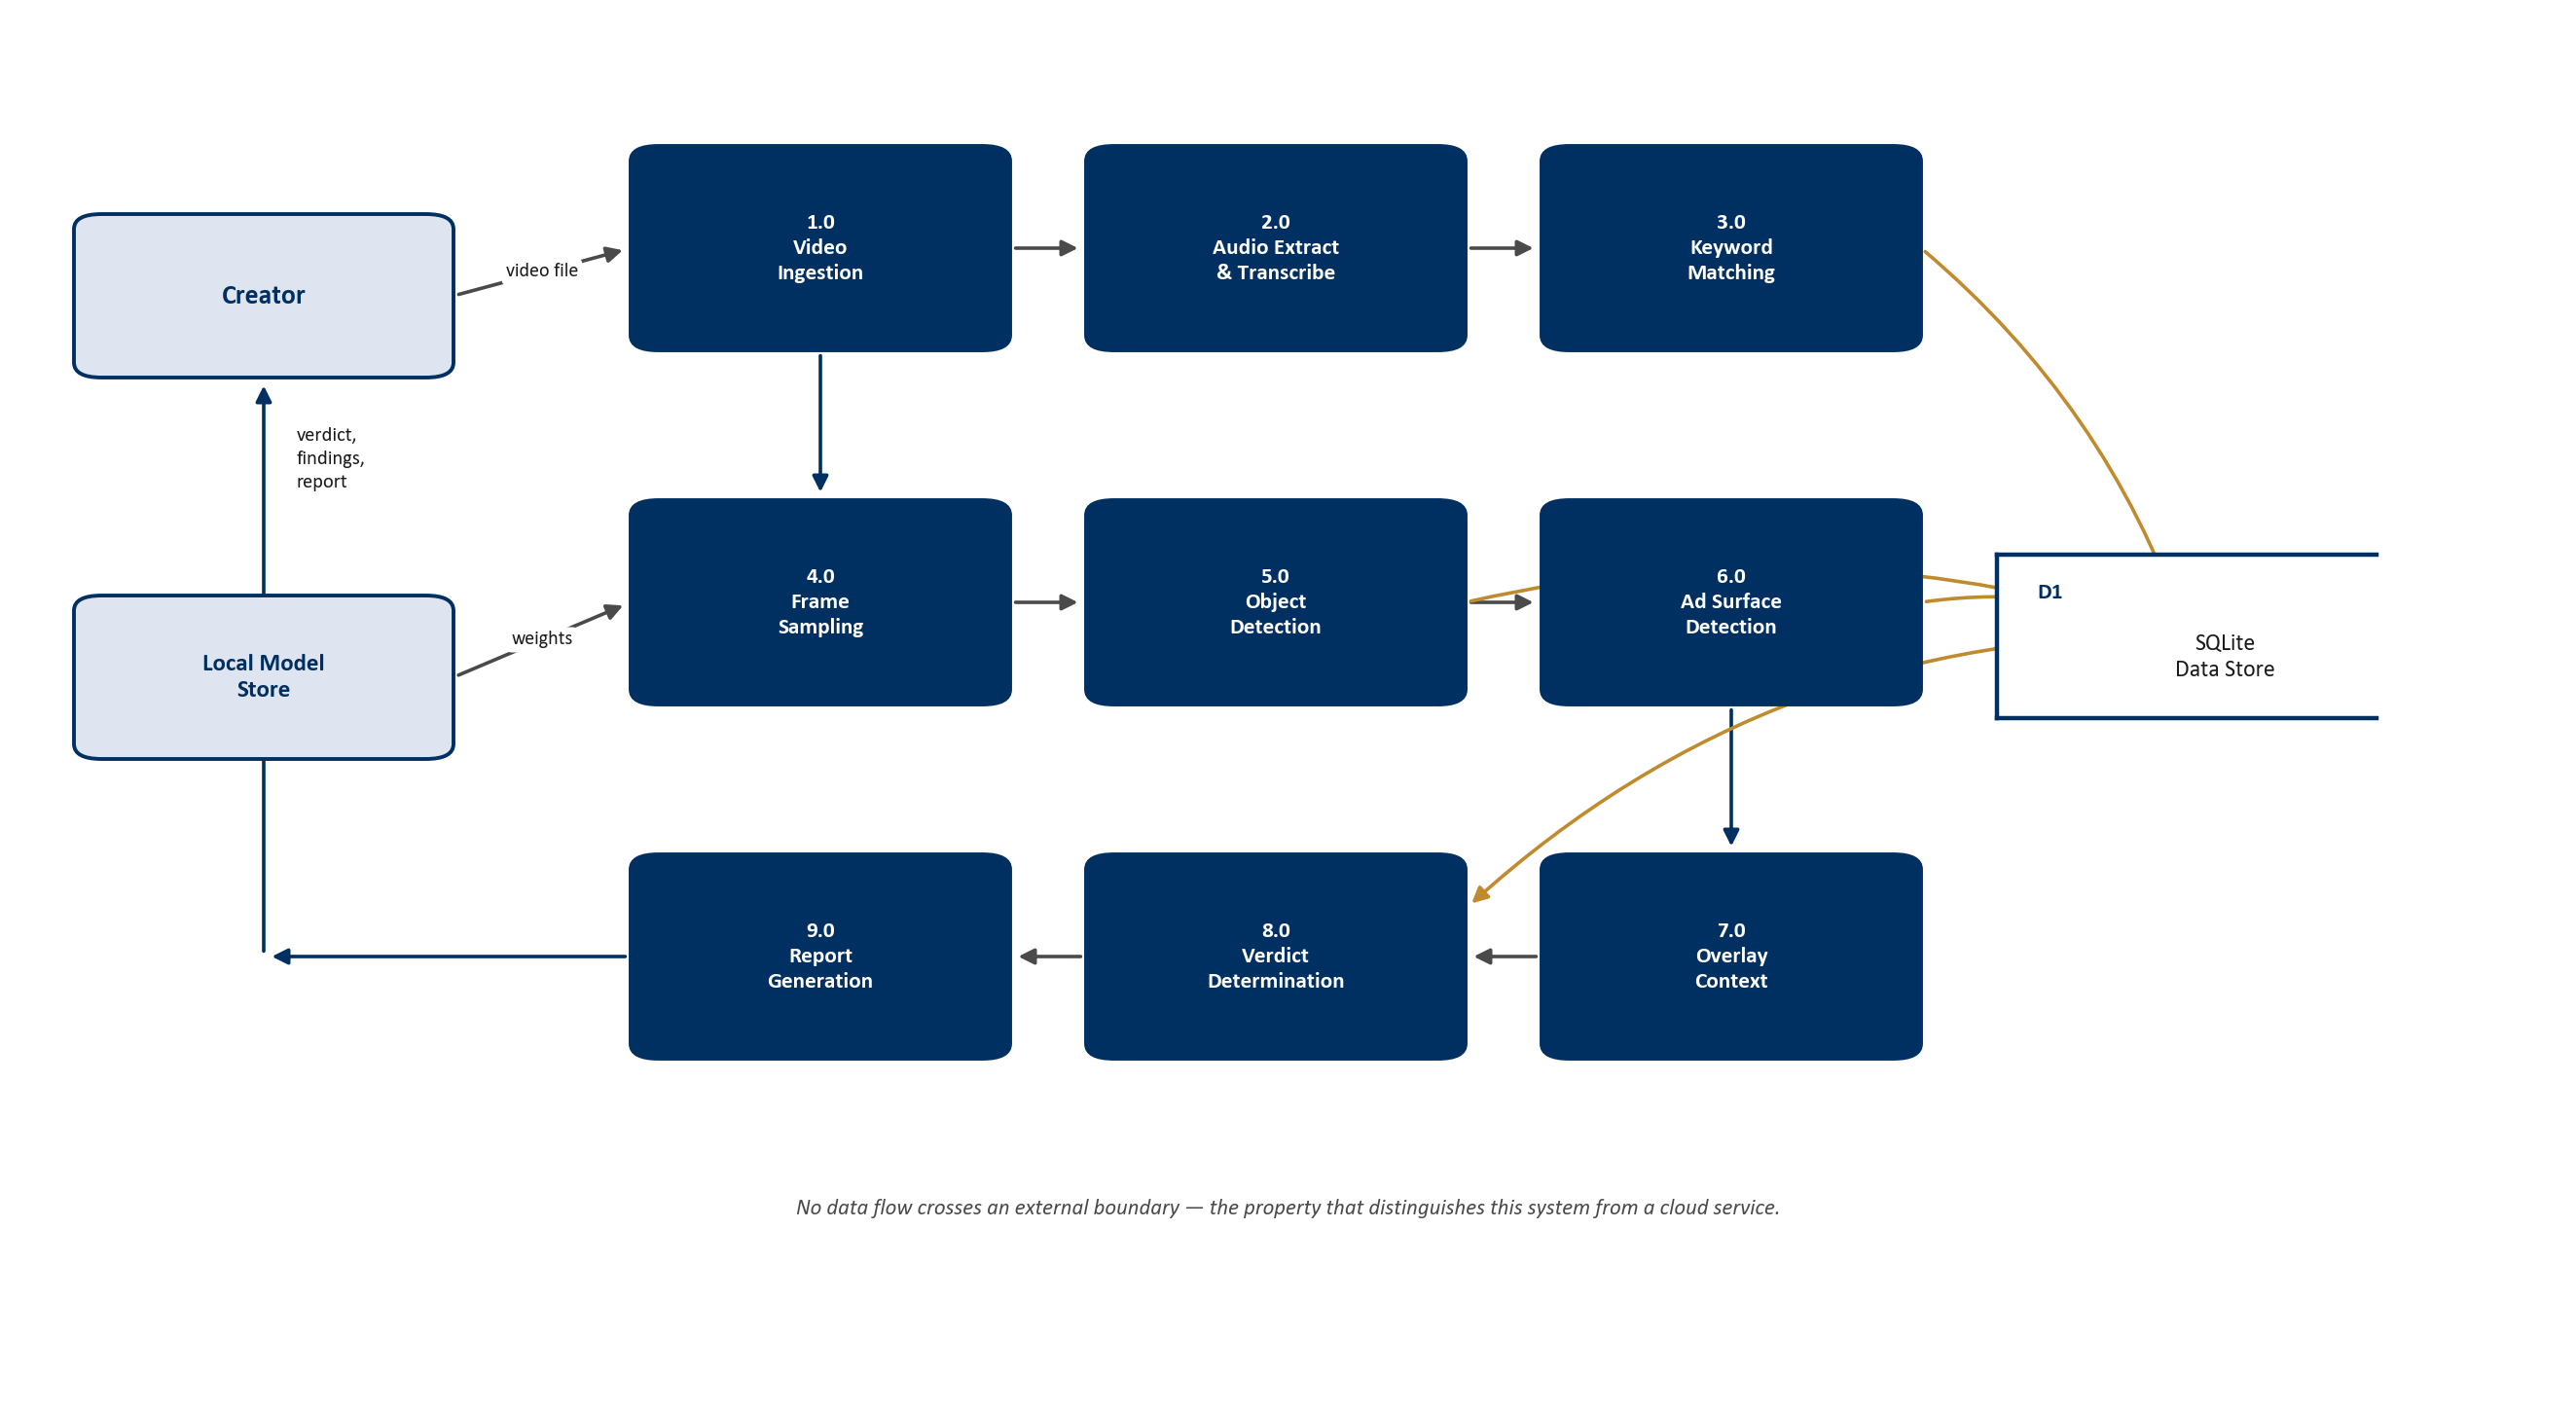
\includegraphics[width=0.95\textwidth]{Images/dfd_level1.png}
\caption{DFD Level 1}
\end{figure}

\subsection*{Explanation}

Video ingestion writes metadata to the data store. Audio and frame processing operate on the stored file and write their findings independently. Verdict determination reads all findings together with the overlay context, which is why it is modelled as a separate process rather than as part of either engine.

\section{Use Case Diagram}

The system has a single actor, the Creator, since it is a single-user offline application.

The use cases are:

\begin{itemize}
\item Upload Video
\item Run Analysis
\item View Findings
\item Navigate Audit Timeline
\item Configure Detection Settings
\item Edit Restricted Dictionary
\item Export Report
\item Delete Video
\end{itemize}

\begin{figure}[H]
\centering
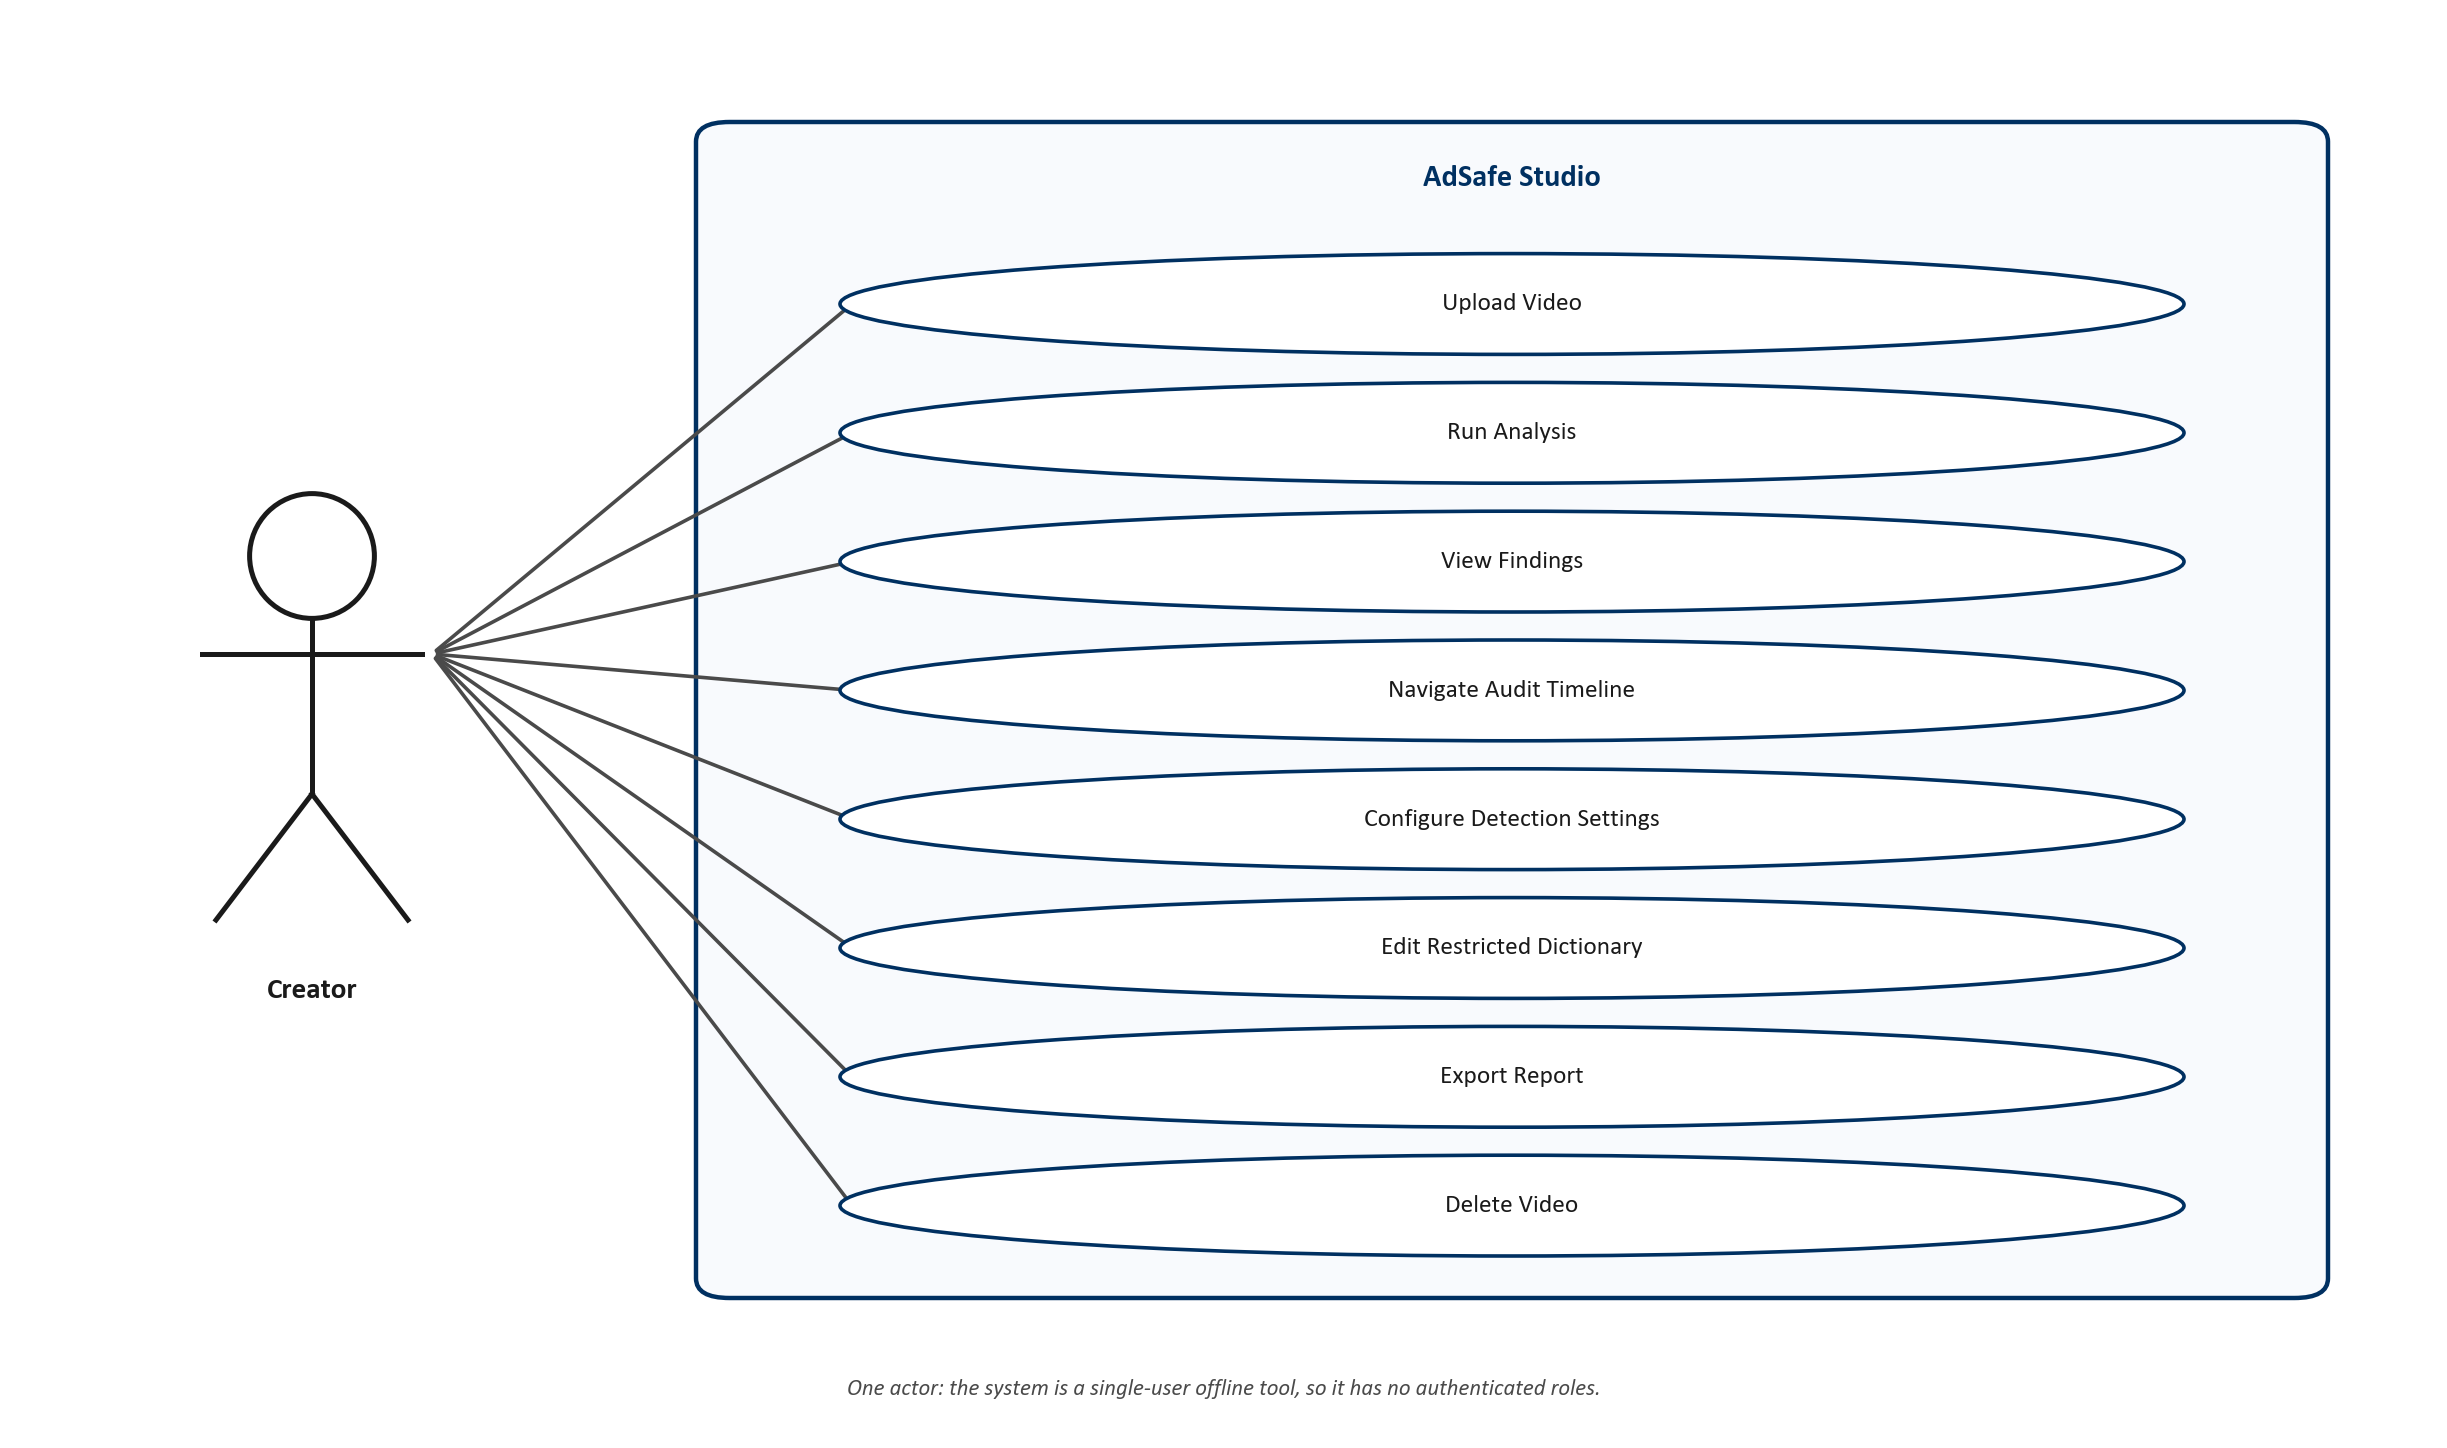
\includegraphics[width=0.92\textwidth]{Images/use_case.png}
\caption{Use Case Diagram}
\end{figure}

\section{Activity Diagram}

The activity diagram describes the sequence of actions performed during an analysis run.

\begin{enumerate}
\item Creator uploads a video.
\item System validates the format and records metadata.
\item Creator starts the analysis.
\item System extracts the audio track.
\item System transcribes the audio and matches restricted terms.
\item System samples frames from the video.
\item System detects risk objects, advertisement surfaces and overlay context from the sampled frames.
\item System merges advertisement surfaces across time.
\item System determines the compliance verdict.
\item System presents findings to the creator.
\end{enumerate}

\begin{figure}[H]
\centering
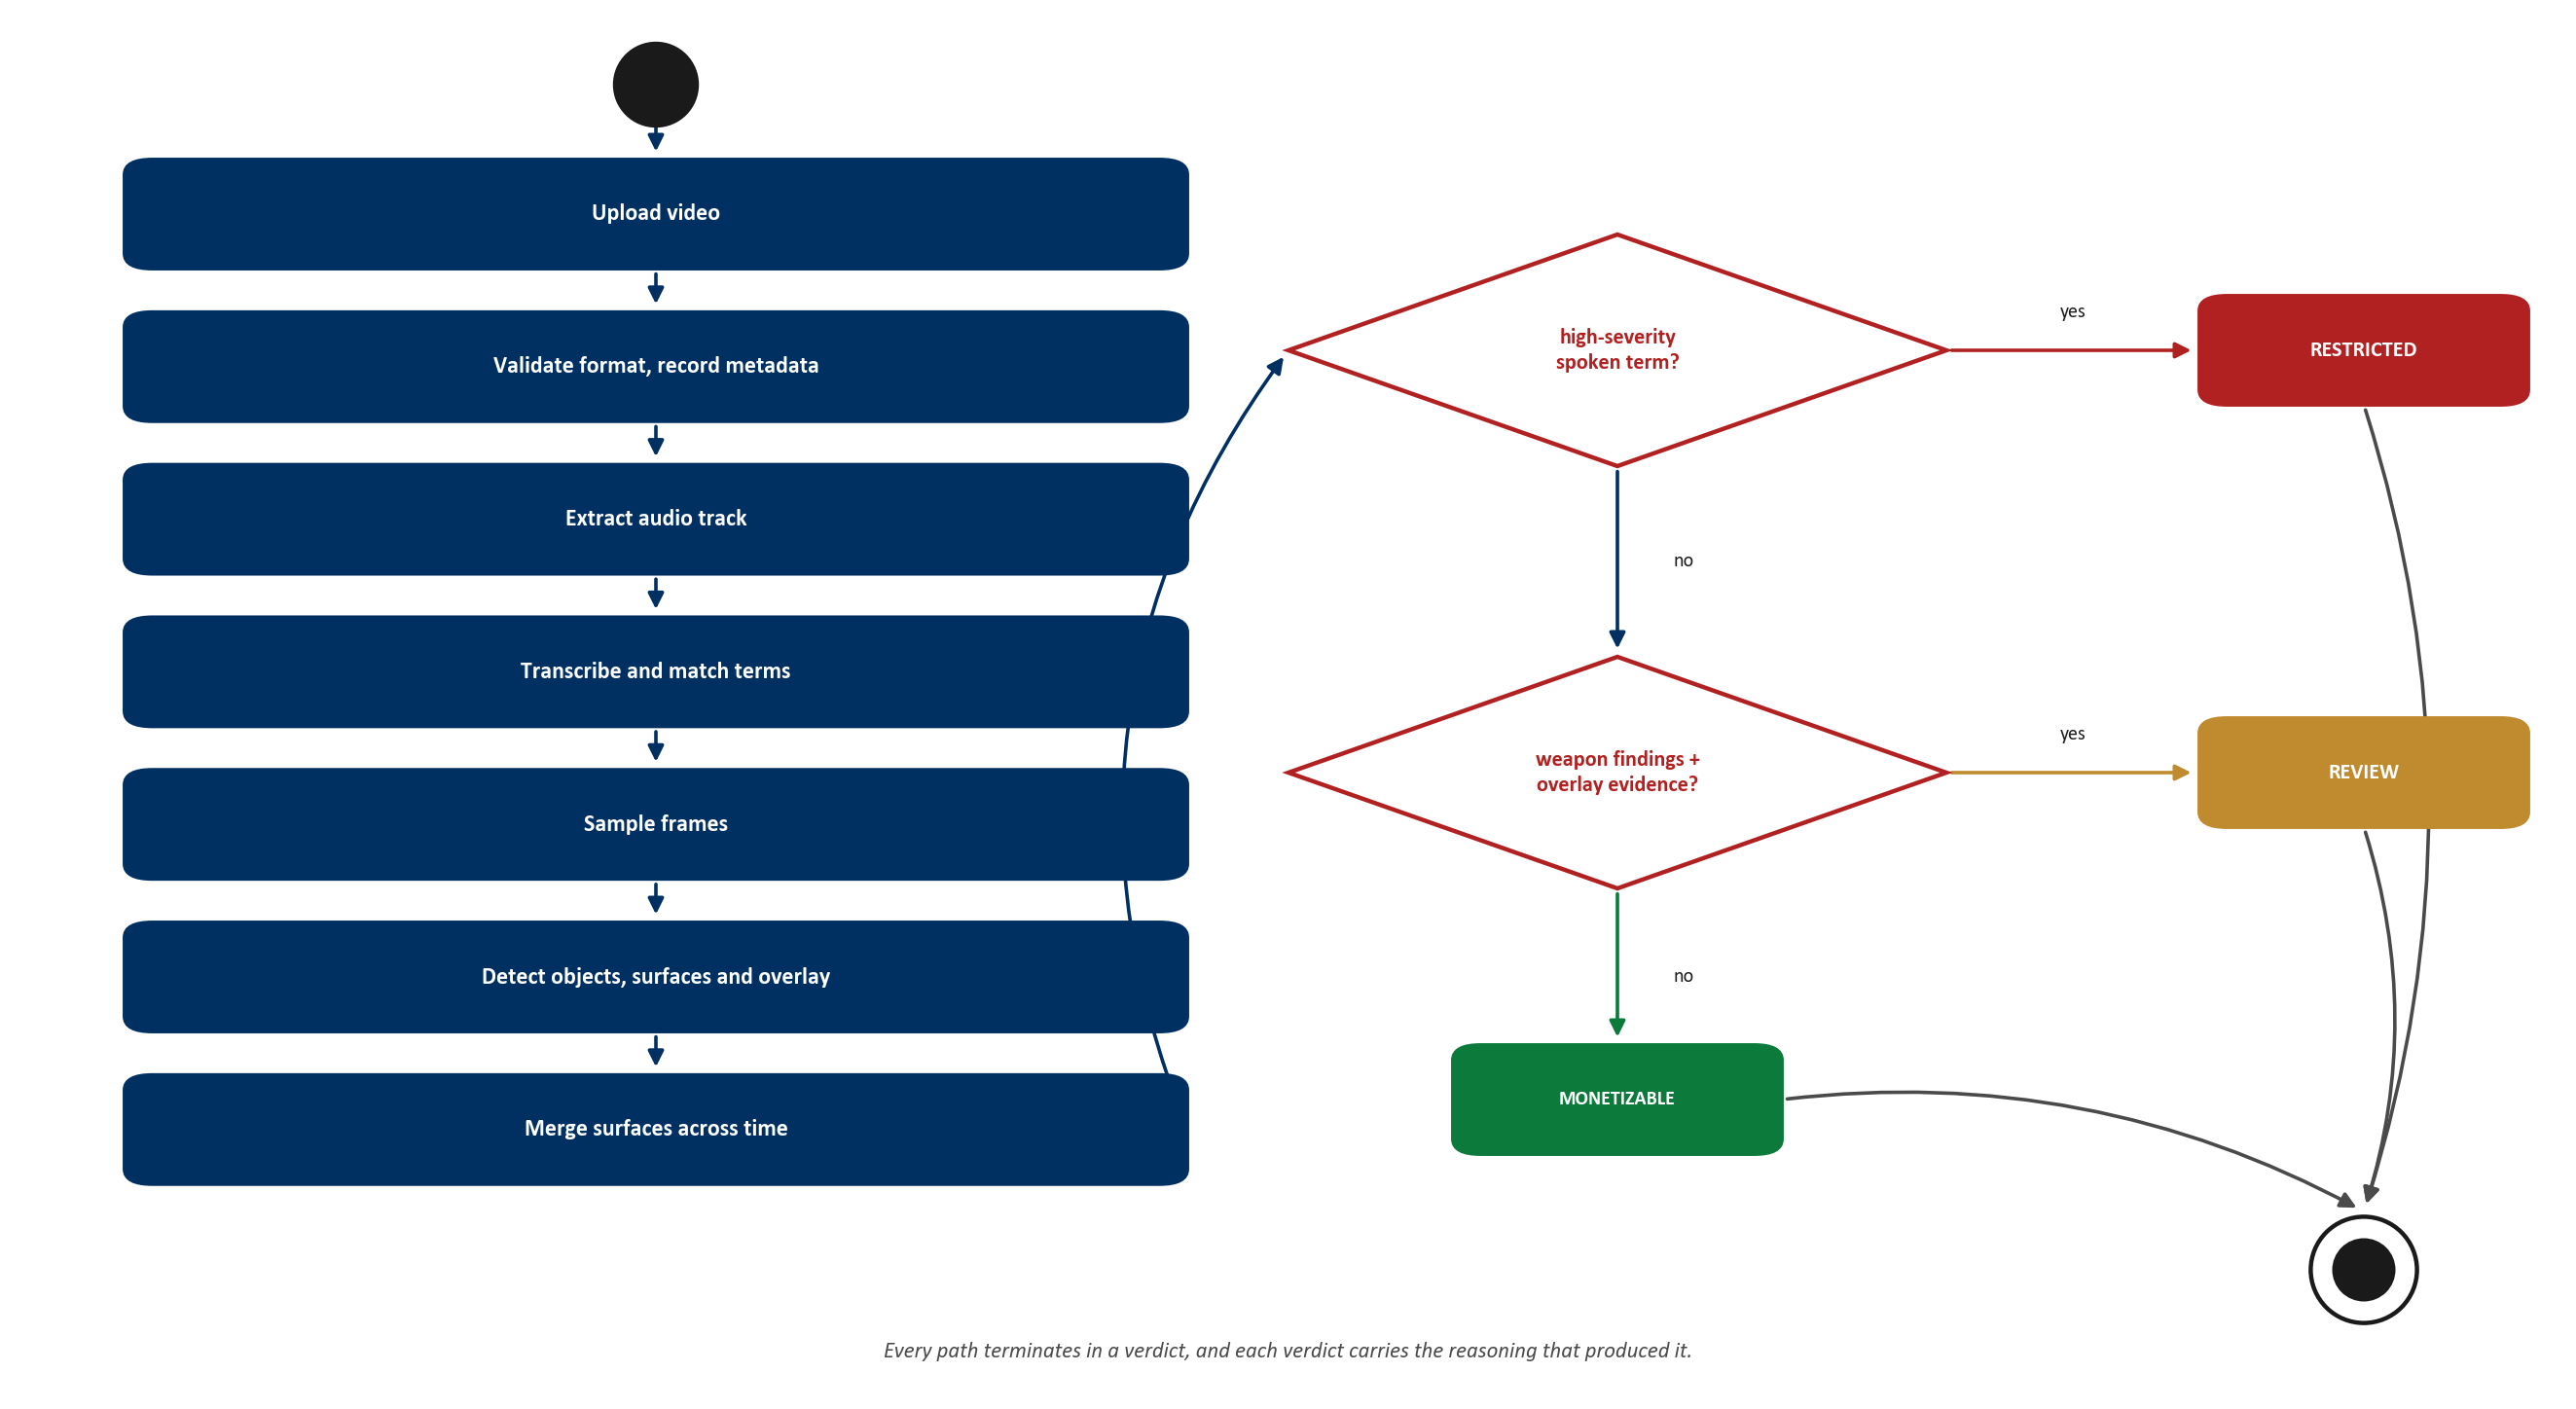
\includegraphics[width=0.88\textwidth]{Images/activity.png}
\caption{Activity Diagram}
\end{figure}

\section{Sequence Diagram}

The sequence diagram describes the interaction between the interface, the API, the orchestrator, the engines and the database during a single analysis.

The interface issues an analysis request to the API, which queues the work in the background and returns immediately so the interface remains responsive. The orchestrator invokes each engine in turn, writing findings to the database, and reports progress that the interface polls until completion.

\begin{figure}[h]
\centering
\fbox{
\parbox{12cm}{
\vspace{7cm}
Sequence Diagram
\vspace{7cm}
}
}
\caption{Sequence Diagram}
\end{figure}

\section{Class Diagram}

The principal classes of the system are:

\begin{table}[h]
\centering
\begin{tabular}{|p{4cm}|p{8cm}|}
\hline
\textbf{Class} & \textbf{Responsibility} \\
\hline
FasterWhisperTranscriber & Transcribes audio into word-level timestamped text \\
\hline
YoloDetector & Runs object detection models over a frame at multiple scales \\
\hline
Detection & One raw model output before risk interpretation \\
\hline
OverlayAccumulator & Accumulates per-pixel statistics across frames \\
\hline
AdSpotParams & Tunable parameters of the free-space algorithm \\
\hline
Orchestrator & Sequences the engines and writes results \\
\hline
Repository & Provides data access over the six tables \\
\hline
\end{tabular}
\caption{Principal Classes}
\end{table}

\begin{figure}[H]
\centering
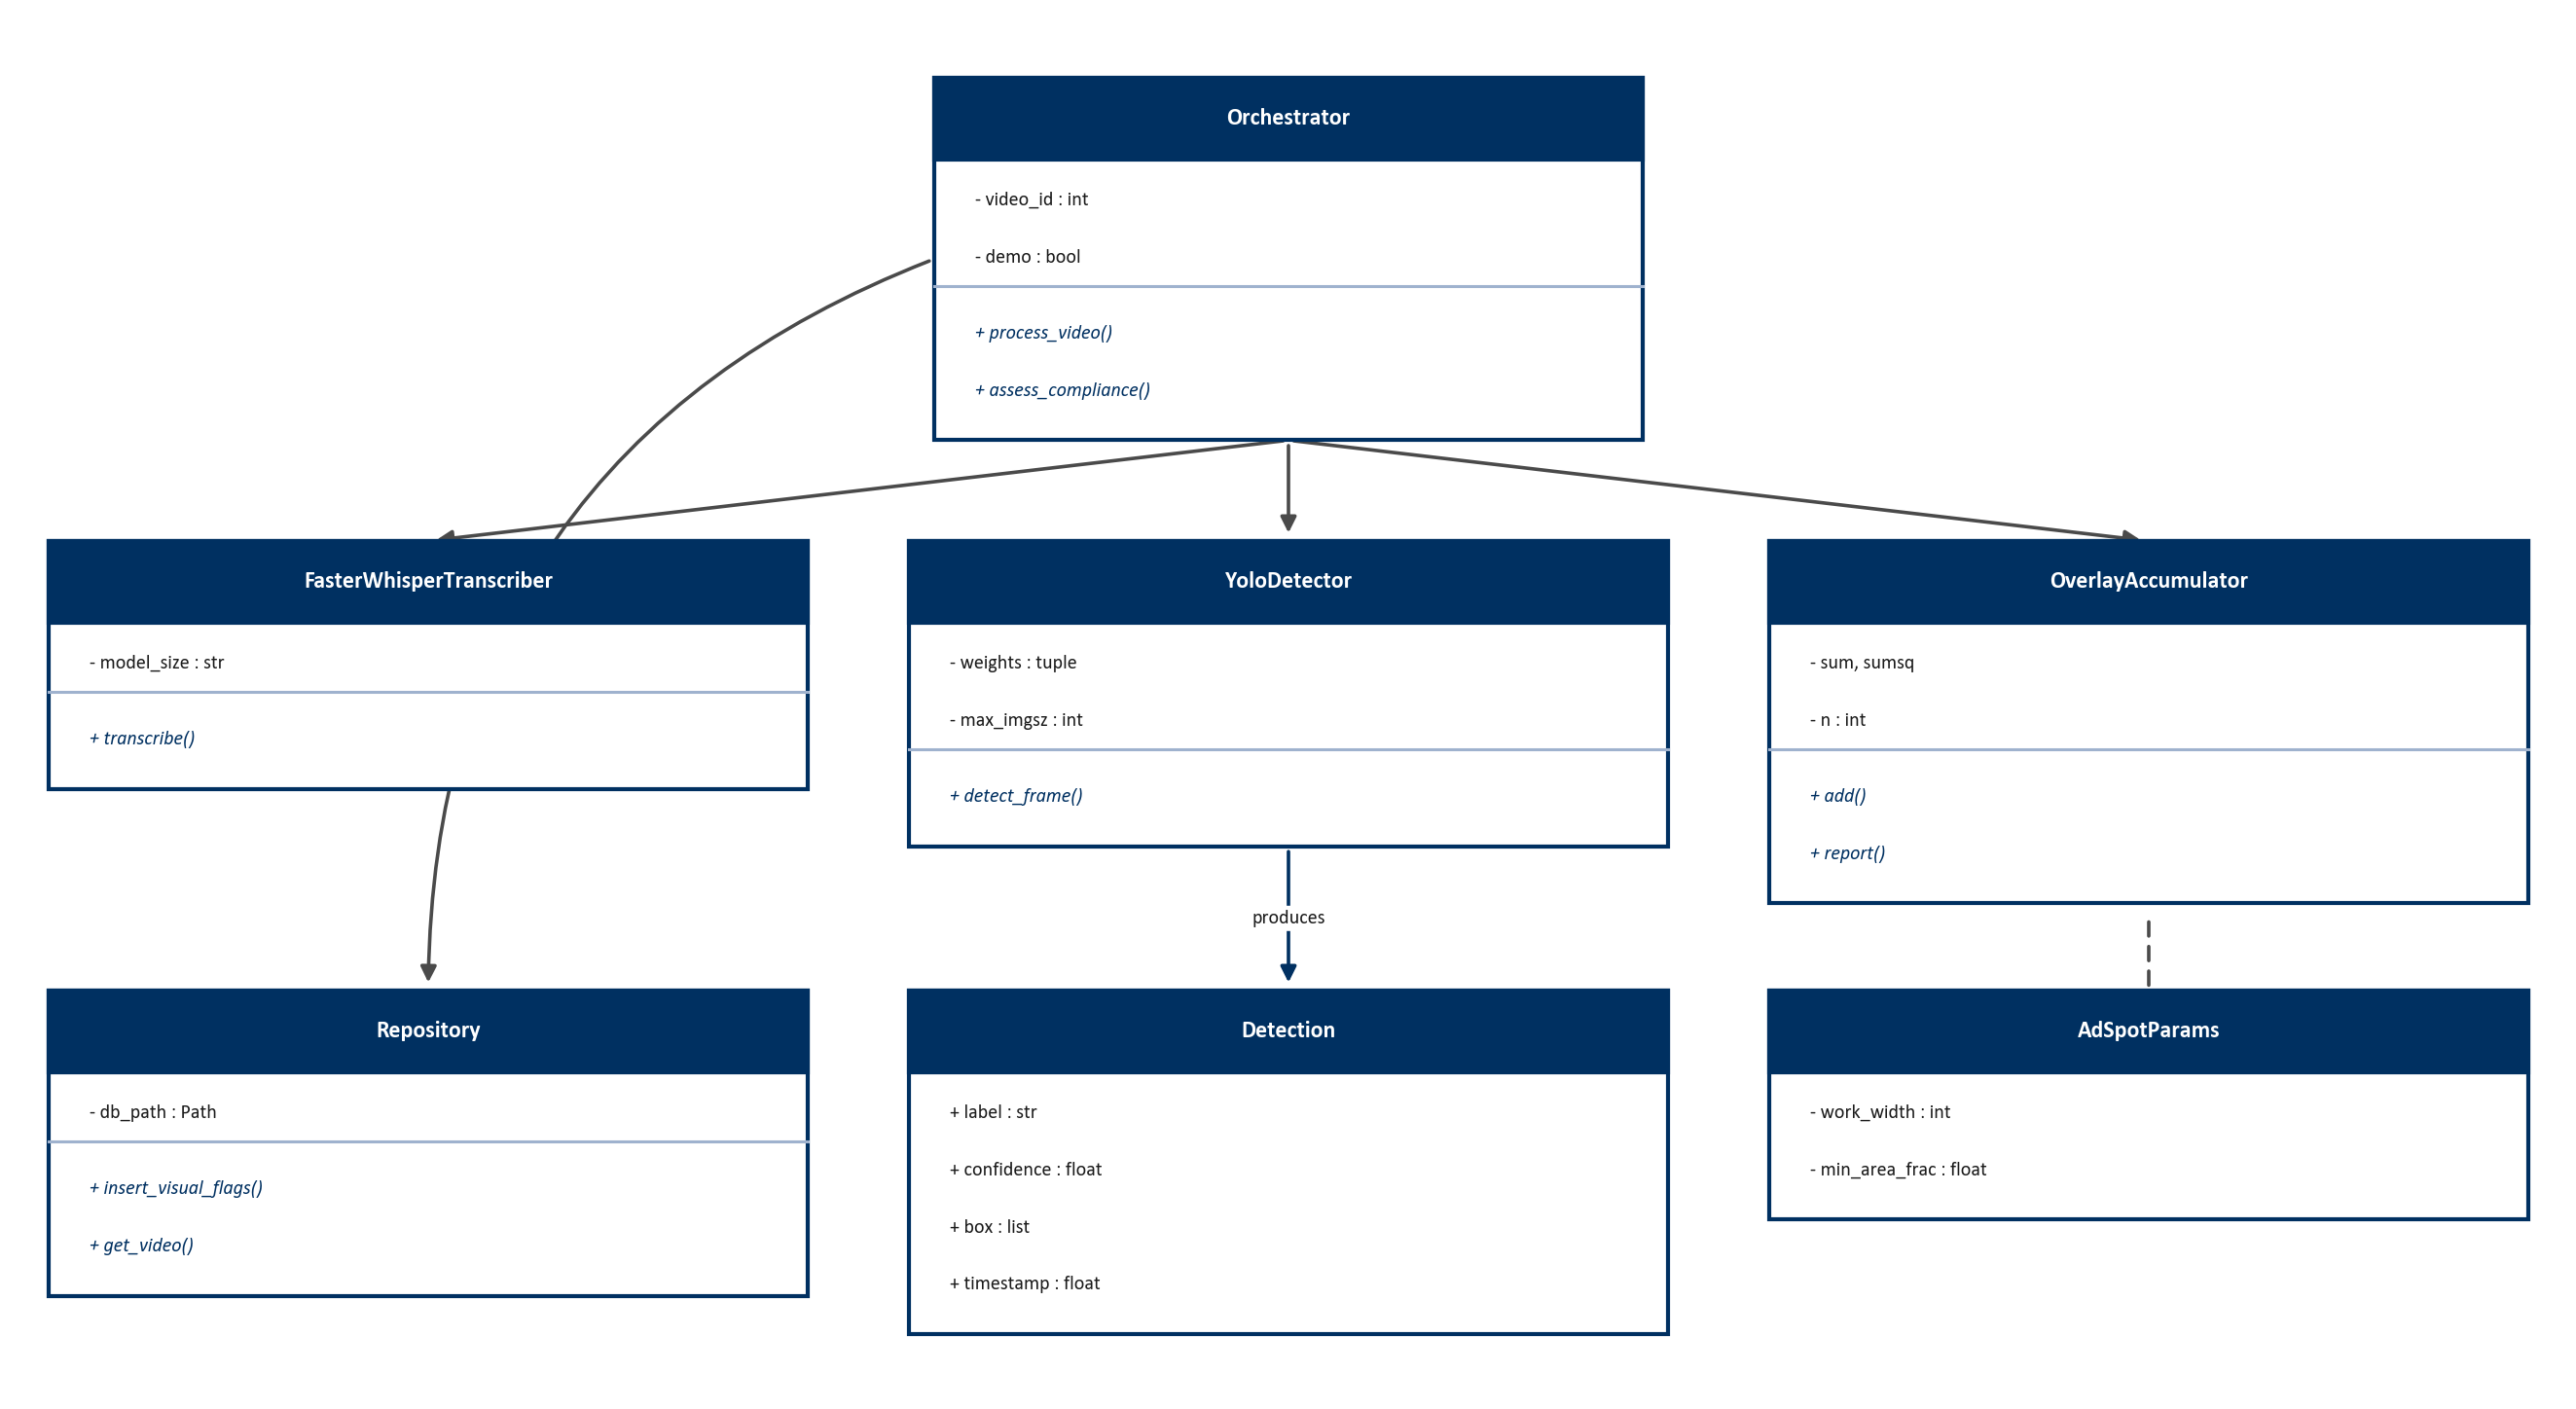
\includegraphics[width=0.95\textwidth]{Images/class_diagram.png}
\caption{Class Diagram}
\end{figure}

\section{Entity Relationship Diagram}

The data model consists of six entities. VideoMetadata is the parent entity; AudioFlags, VisualFlags, AdSpots and AuditReports are each dependent on it through a one-to-many relationship. SystemConfig is independent and holds application settings.

\begin{table}[h]
\centering
\begin{tabular}{|p{4cm}|p{4cm}|p{4cm}|}
\hline
\textbf{Parent} & \textbf{Child} & \textbf{Cardinality} \\
\hline
VideoMetadata & AudioFlags & One to Many \\
\hline
VideoMetadata & VisualFlags & One to Many \\
\hline
VideoMetadata & AdSpots & One to Many \\
\hline
VideoMetadata & AuditReports & One to Many \\
\hline
\end{tabular}
\caption{Entity Relationships}
\end{table}

\begin{figure}[H]
\centering
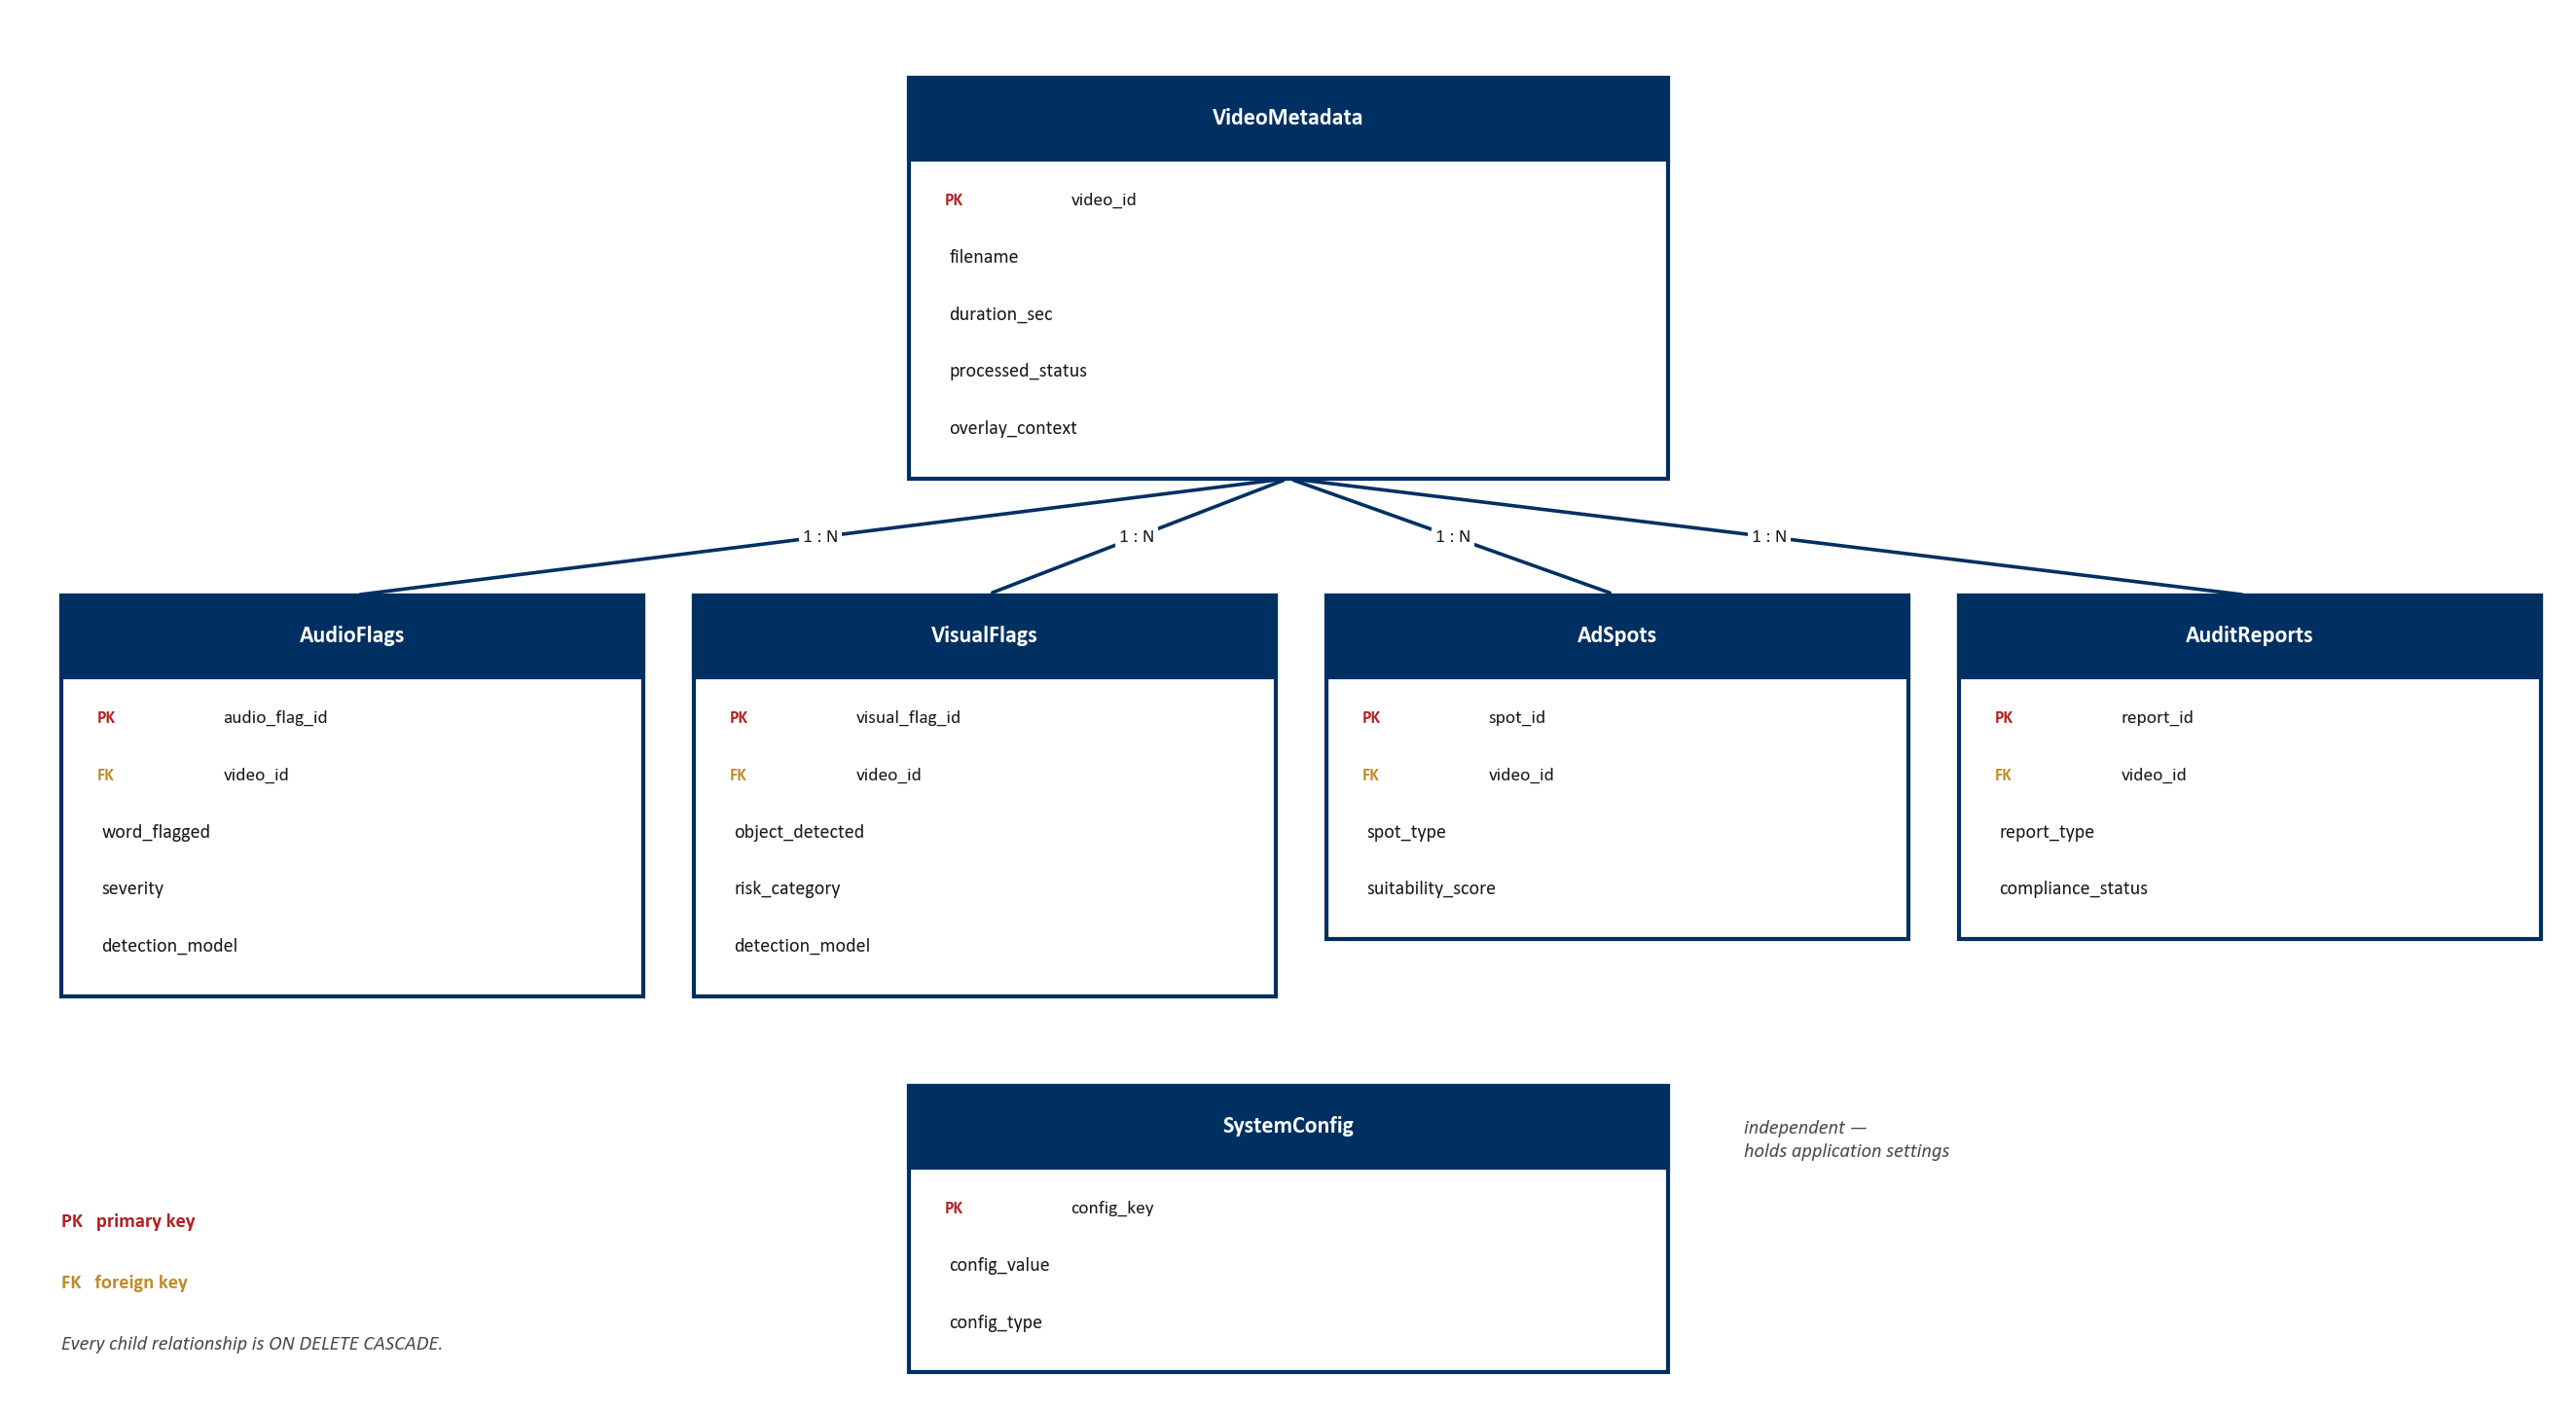
\includegraphics[width=0.95\textwidth]{Images/er_diagram.png}
\caption{Entity Relationship Diagram}
\end{figure}

\section{Chapter Summary}

This chapter presented the structural and behavioural models of the system. The data flow models establish that no data crosses an external boundary. The sequence model records that analysis runs in the background so the interface remains responsive. The entity relationship model shows a single parent entity with four dependent finding types, which allows all findings for a video to be removed by deleting the video itself.

%%%%%%%%%%%%%%%%%%%%%%%%%%%%%%%%%%%%%%%%%%%%%%%%%%
\chapter{System Design}
%%%%%%%%%%%%%%%%%%%%%%%%%%%%%%%%%%%%%%%%%%%%%%%%%%

\section{Introduction}

This chapter describes the architecture of the system, the division of responsibility between its modules, the design of the database, and the design of the user interface.

\section{System Architecture}

The system follows a four-layer architecture consisting of a presentation layer, a controller layer, an artificial intelligence engine layer and a data layer.

\begin{table}[h]
\centering
\begin{tabular}{|p{3.5cm}|p{8.5cm}|}
\hline
\textbf{Layer} & \textbf{Responsibility} \\
\hline
Presentation & React application providing seven screens and the audit timeline \\
\hline
Controller & FastAPI application exposing fifteen REST endpoints and serving media \\
\hline
AI Engine & Transcription, object detection, advertisement placement and overlay analysis \\
\hline
Data & SQLite database with write-ahead logging and enforced foreign keys \\
\hline
\end{tabular}
\caption{Architectural Layers}
\end{table}

\begin{figure}[H]
\centering
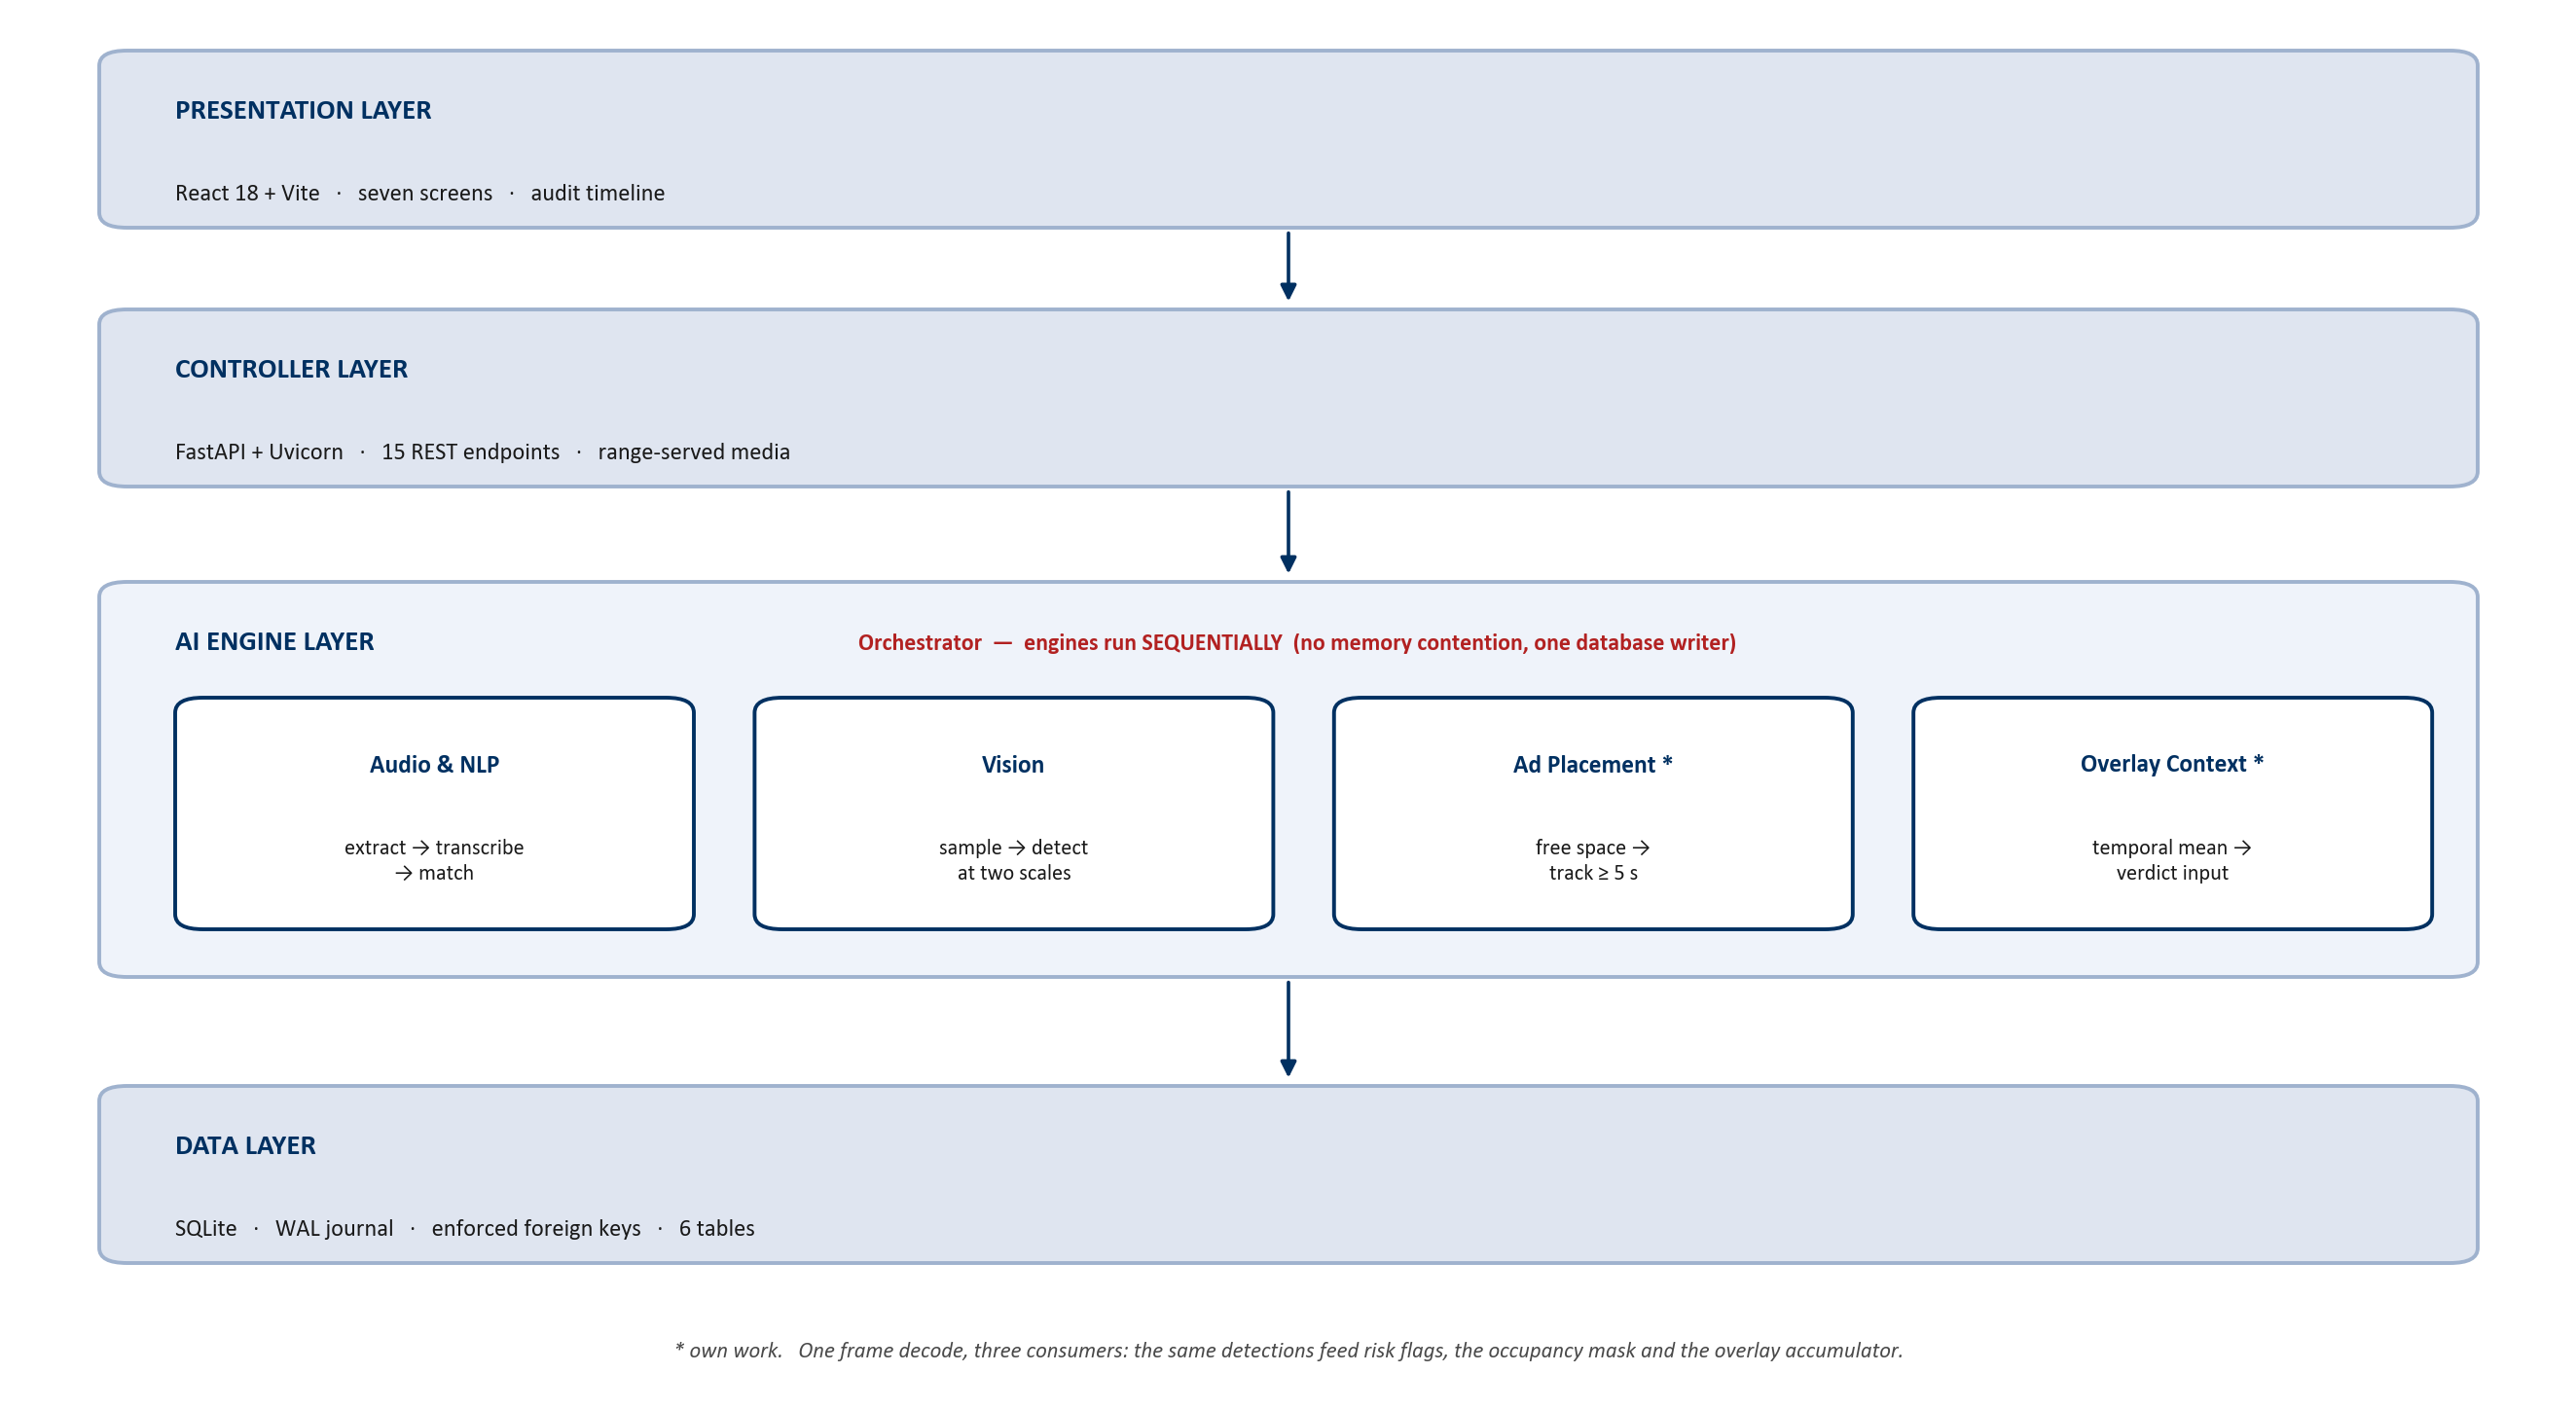
\includegraphics[width=0.95\textwidth]{Images/architecture.png}
\caption{System Architecture}
\end{figure}

\subsection{Sequential Processing}

The engines execute sequentially rather than in parallel. Three considerations determine this.

\begin{itemize}
\item The transcription and detection models contend for the same system memory, and running them together degrades both.
\item Concurrent writers to a single SQLite database produce lock contention.
\item The interpreter's global lock limits genuine parallelism for computation-bound work in any case.
\end{itemize}

Write-ahead logging is enabled so that interface queries never block the single writer.

\subsection{Single Decode, Three Consumers}

Each sampled frame is decoded once and used by three consumers: risk detection, advertisement surface detection and overlay accumulation. The object detections that identify risks also define the occupancy mask required by the placement algorithm, so no additional inference is performed. Overlay detection requires the whole frame sequence rather than a single image, but accumulates in constant memory and therefore adds a running total per frame rather than a second pass over the file.

\section{Modularization Details}

\subsection{Audio and Natural Language Module}

Responsible for recovering spoken content and identifying restricted terminology.

\begin{itemize}
\item Extracts the audio track to 16 kHz mono using a bundled encoder.
\item Transcribes with word-level timestamps.
\item Matches the transcript against the configured dictionary using word-boundary and phrase matching.
\item Records the producing model against every finding.
\end{itemize}

\subsection{Vision Module}

Responsible for visual risk detection.

\begin{itemize}
\item Samples frames by seeking rather than decoding every frame.
\item Runs detection at two resolutions and merges the results.
\item Normalises model class names into the system's risk categories.
\item Reports what the loaded models are actually capable of detecting.
\end{itemize}

\subsection{Advertisement Placement Module}

Responsible for identifying placement surfaces.

\begin{itemize}
\item Builds an occupancy mask from detected objects.
\item Builds a texture mask from edge density and local variance.
\item Locates the largest rectangles within the remaining free area.
\item Scores each surface on area, uniformity and centrality.
\end{itemize}

\subsection{Overlay Context Module}

Responsible for distinguishing rendered from filmed content.

\begin{itemize}
\item Accumulates per-pixel temporal statistics across sampled frames.
\item Identifies structure that persists while the scene behind it changes.
\item Declines to reach a conclusion when the scene is largely static.
\end{itemize}

\subsection{Orchestration Module}

Responsible for sequencing the analysis and recording its results.

\begin{itemize}
\item Selects the engine for each stage independently.
\item Reports progress during processing.
\item Clears previous findings before re-analysis so runs are idempotent.
\item Records the engine that produced each result.
\end{itemize}

\subsection{Reporting Module}

Responsible for exporting findings.

\begin{itemize}
\item Produces PDF, CSV and JSON output.
\item Draws a timeline of findings in the PDF report.
\item States provenance on every report.
\item Records generated reports in the archive table.
\end{itemize}

\section{Data Integrity and Constraints}

\subsection{Primary Key Constraints}

Every table declares a primary key. Finding tables use an auto-incrementing integer identifier; the configuration table is keyed by its setting name.

\subsection{Foreign Key Constraints}

Every finding table references VideoMetadata with cascading deletion, so removing a video removes all of its findings and leaves no orphaned rows. Foreign key enforcement is enabled explicitly on each connection, as the database engine disables it by default.

\subsection{Check Constraints}

Constrained columns reject invalid values at the database level rather than relying on application code:

\begin{itemize}
\item Processing status is restricted to pending, processing, completed or failed.
\item Severity is restricted to Low, Medium or High.
\item Risk category is restricted to Weapon, Substance or Graphic.
\item Report type is restricted to PDF, CSV or JSON.
\end{itemize}

\subsection{Not Null Constraints}

Columns without which a record has no meaning are declared not null, including file path, duration, timestamps, detected object and confidence score.

\section{Database Design}

The database consists of six tables in third normal form.

\subsection{VideoMetadata Table}

\begin{table}[h]
\centering
\begin{tabular}{|p{4cm}|p{2.5cm}|p{5cm}|}
\hline
\textbf{Column} & \textbf{Type} & \textbf{Description} \\
\hline
video\_id & INTEGER & Primary key \\
\hline
filename & TEXT & Original file name \\
\hline
filepath & TEXT & Stored location \\
\hline
file\_size\_mb & REAL & File size \\
\hline
duration\_sec & REAL & Duration in seconds \\
\hline
fps & REAL & Frame rate \\
\hline
resolution\_width & INTEGER & Frame width \\
\hline
resolution\_height & INTEGER & Frame height \\
\hline
upload\_timestamp & TEXT & Time of ingestion \\
\hline
processed\_status & TEXT & Analysis state \\
\hline
overlay\_context & TEXT & Overlay evidence as JSON \\
\hline
\end{tabular}
\caption{VideoMetadata Table}
\end{table}

\subsection{AudioFlags Table}

\begin{table}[h]
\centering
\begin{tabular}{|p{4cm}|p{2.5cm}|p{5cm}|}
\hline
\textbf{Column} & \textbf{Type} & \textbf{Description} \\
\hline
audio\_flag\_id & INTEGER & Primary key \\
\hline
video\_id & INTEGER & Foreign key \\
\hline
timestamp\_start & REAL & Start of the spoken term \\
\hline
timestamp\_end & REAL & End of the spoken term \\
\hline
word\_flagged & TEXT & Matched term \\
\hline
transcript\_context & TEXT & Surrounding transcript \\
\hline
severity & TEXT & Low, Medium or High \\
\hline
detection\_model & TEXT & Producing engine \\
\hline
\end{tabular}
\caption{AudioFlags Table}
\end{table}

\subsection{VisualFlags Table}

\begin{table}[h]
\centering
\begin{tabular}{|p{4cm}|p{2.5cm}|p{5cm}|}
\hline
\textbf{Column} & \textbf{Type} & \textbf{Description} \\
\hline
visual\_flag\_id & INTEGER & Primary key \\
\hline
video\_id & INTEGER & Foreign key \\
\hline
frame\_timestamp & REAL & Position in the video \\
\hline
object\_detected & TEXT & Model class name \\
\hline
bounding\_box\_json & TEXT & Region within the frame \\
\hline
confidence\_score & REAL & Detection confidence \\
\hline
risk\_category & TEXT & Weapon, Substance or Graphic \\
\hline
detection\_model & TEXT & Producing engine \\
\hline
\end{tabular}
\caption{VisualFlags Table}
\end{table}

\subsection{AdSpots Table}

\begin{table}[h]
\centering
\begin{tabular}{|p{4cm}|p{2.5cm}|p{5cm}|}
\hline
\textbf{Column} & \textbf{Type} & \textbf{Description} \\
\hline
spot\_id & INTEGER & Primary key \\
\hline
video\_id & INTEGER & Foreign key \\
\hline
timestamp\_start & REAL & Start of the surface \\
\hline
timestamp\_end & REAL & End of the surface \\
\hline
spot\_type & TEXT & Classified surface type \\
\hline
bounding\_box\_json & TEXT & Region within the frame \\
\hline
area\_pixels & REAL & Surface area \\
\hline
suitability\_score & REAL & Placement suitability \\
\hline
\end{tabular}
\caption{AdSpots Table}
\end{table}

\subsection{AuditReports and SystemConfig Tables}

AuditReports records each generated report with its type, file path, finding totals and compliance status. SystemConfig holds application settings as typed key-value pairs, including the restricted dictionary, sampling rate, confidence threshold, detection resolution cap, analysis mode and the list of active model weights.

\section{User Interface Design}

The interface consists of seven screens and follows conventions established by existing video management tools, so that the layout is familiar to the intended user.

\subsection{Dashboard Screen}

Presents library-wide totals, the distribution of compliance verdicts and recent uploads.

\begin{figure}[H]
\centering
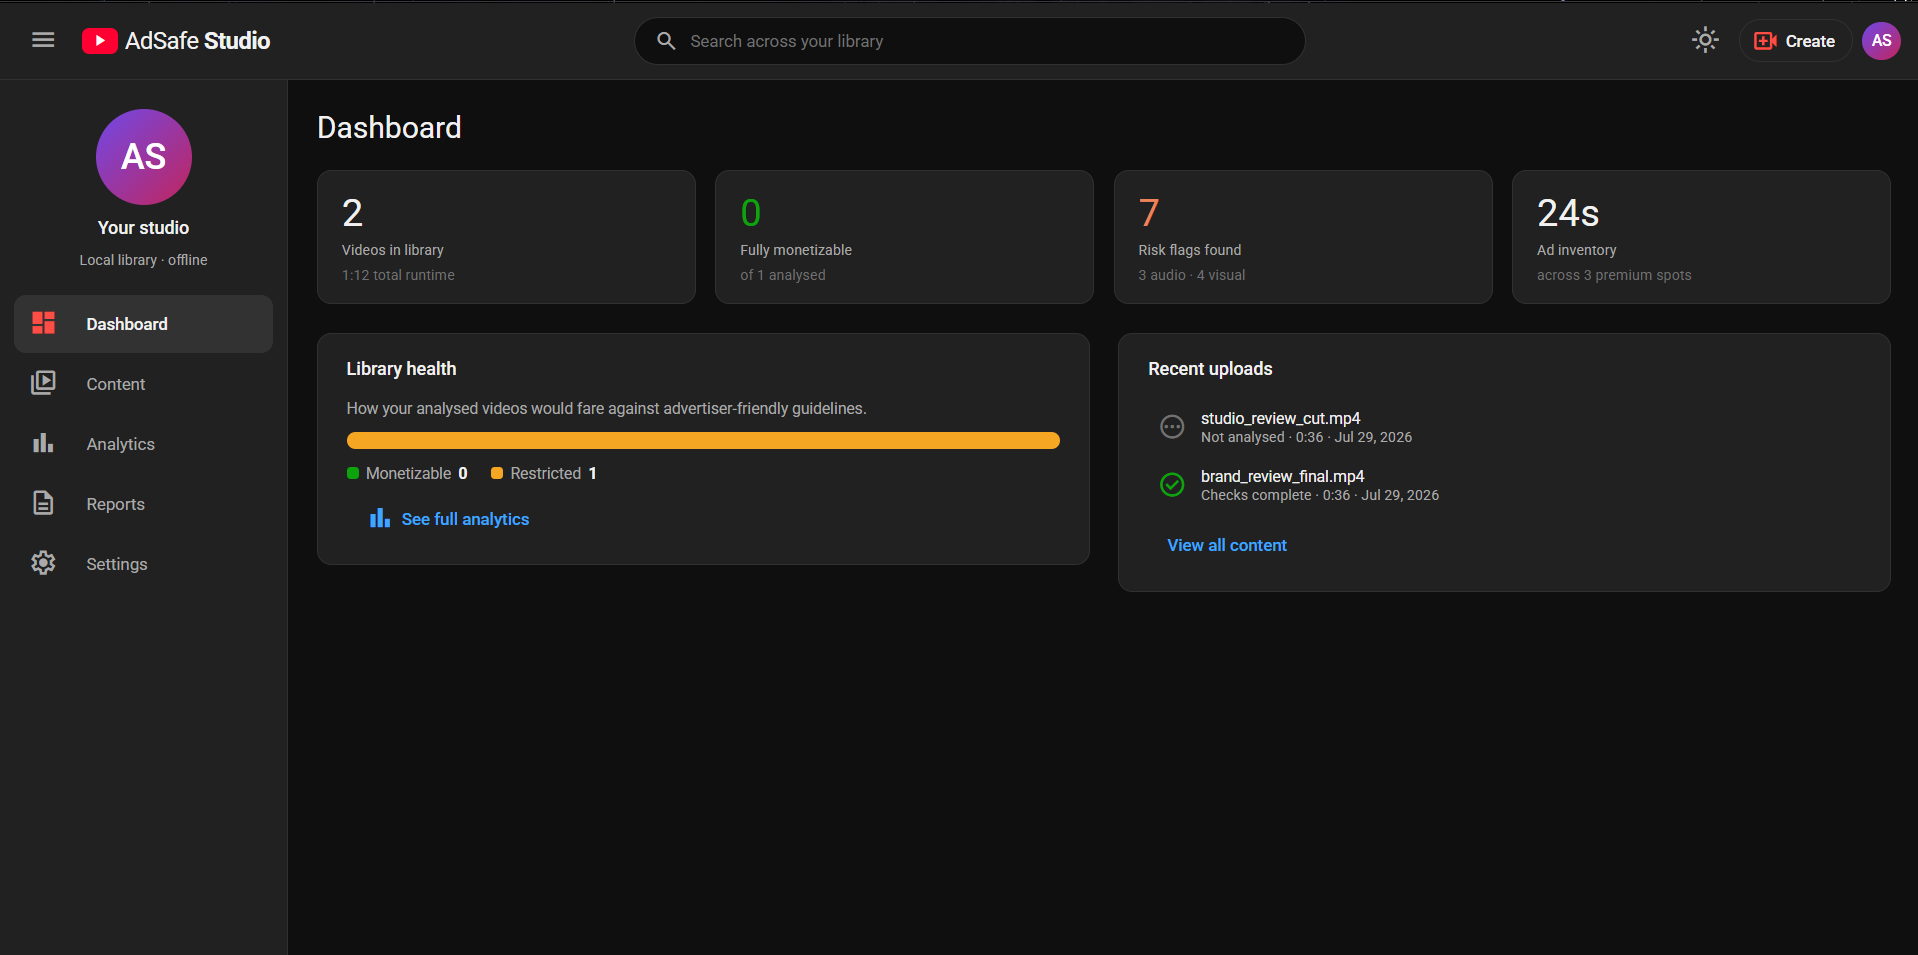
\includegraphics[width=0.95\textwidth]{Images/01-dashboard.png}
\caption{Dashboard Screen}
\end{figure}

\subsection{Content Screen}

Lists all videos with thumbnails, monetization status, finding counts and live analysis progress.

\begin{figure}[H]
\centering
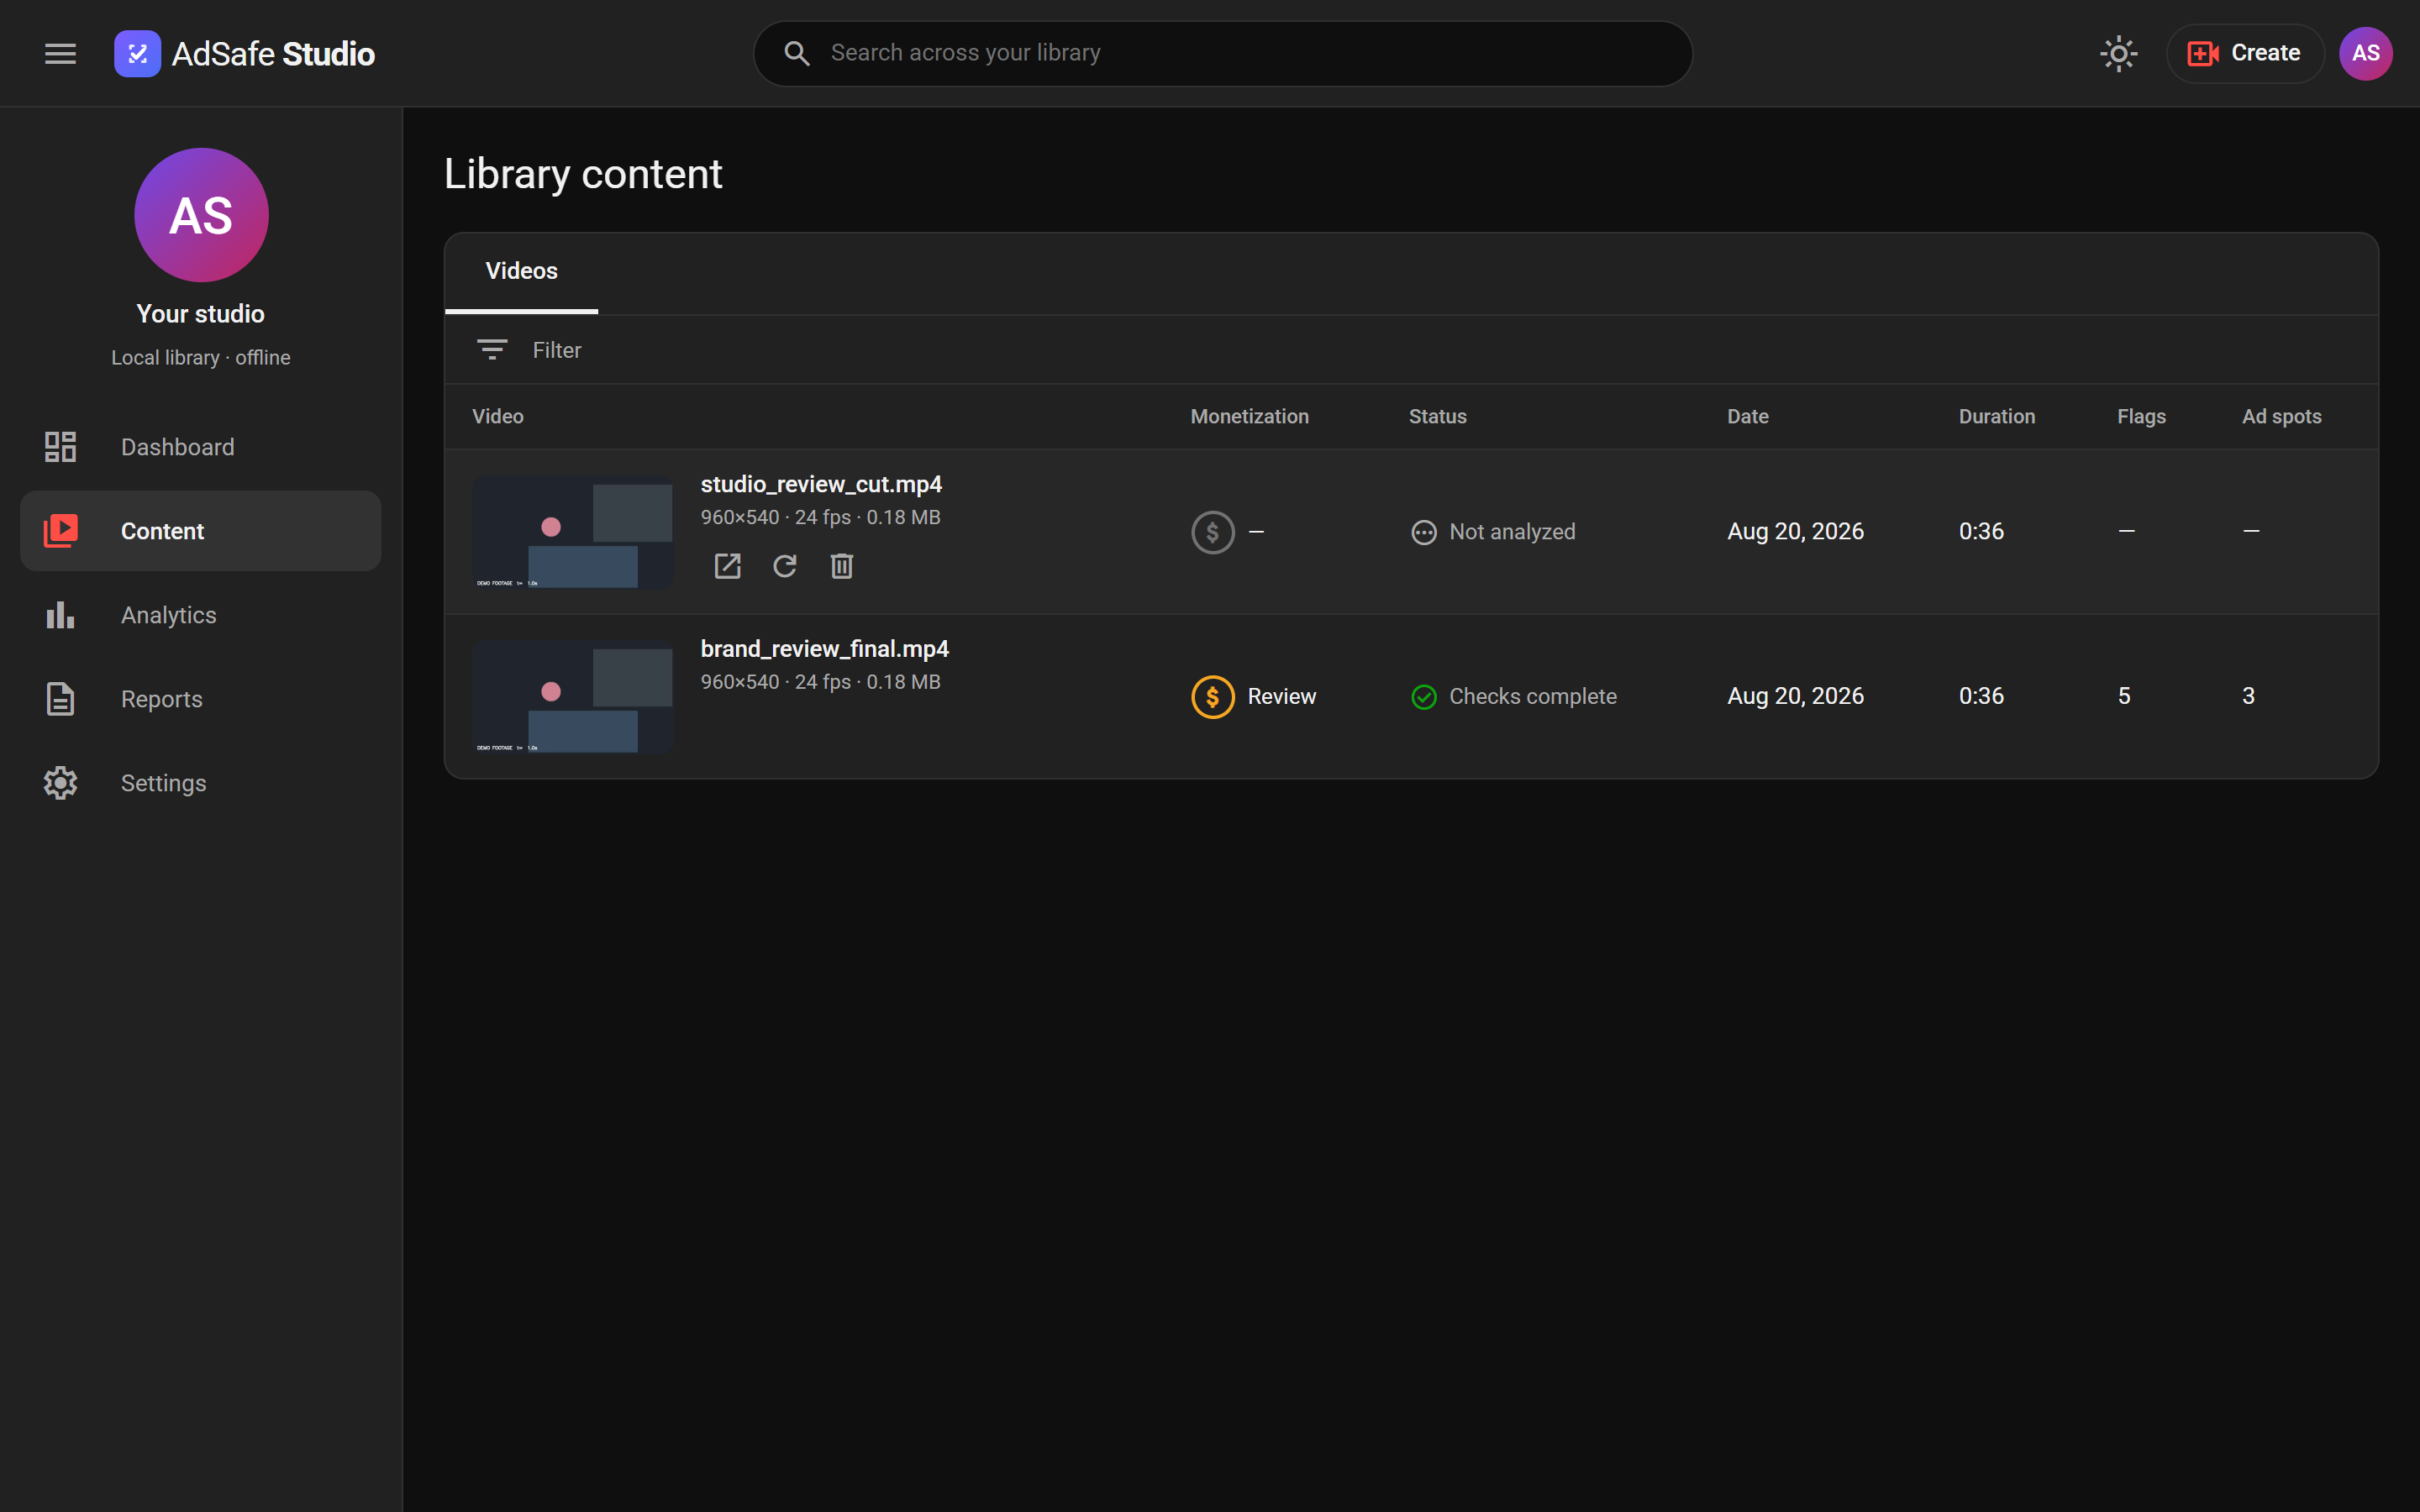
\includegraphics[width=0.95\textwidth]{Images/02-content.png}
\caption{Content Screen}
\end{figure}

\subsection{Video Detail Screen}

Presents the video player alongside the audit timeline and the tables of findings. Selecting any finding moves the player to that position.

\begin{figure}[H]
\centering
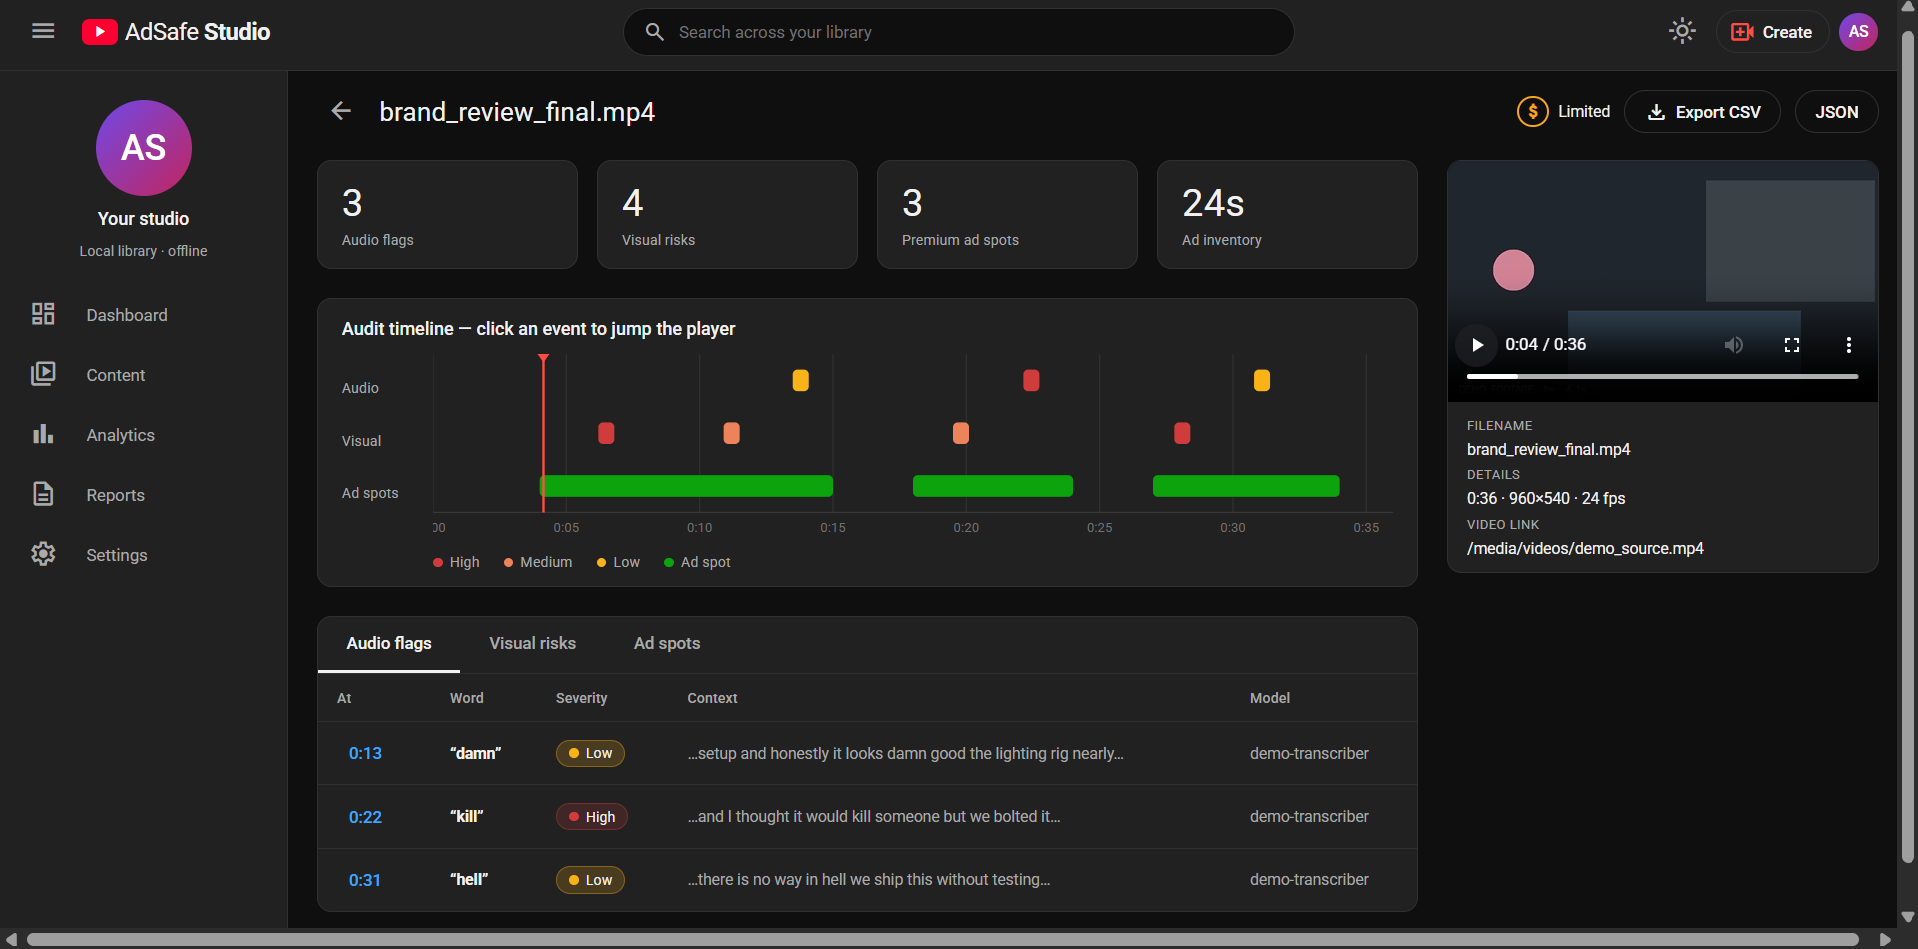
\includegraphics[width=0.95\textwidth]{Images/03-video-detail.png}
\caption{Video Detail Screen}
\end{figure}

\subsection{Reports Screen}

Allows reports to be generated in each supported format and lists previously generated reports for download.

\begin{figure}[H]
\centering
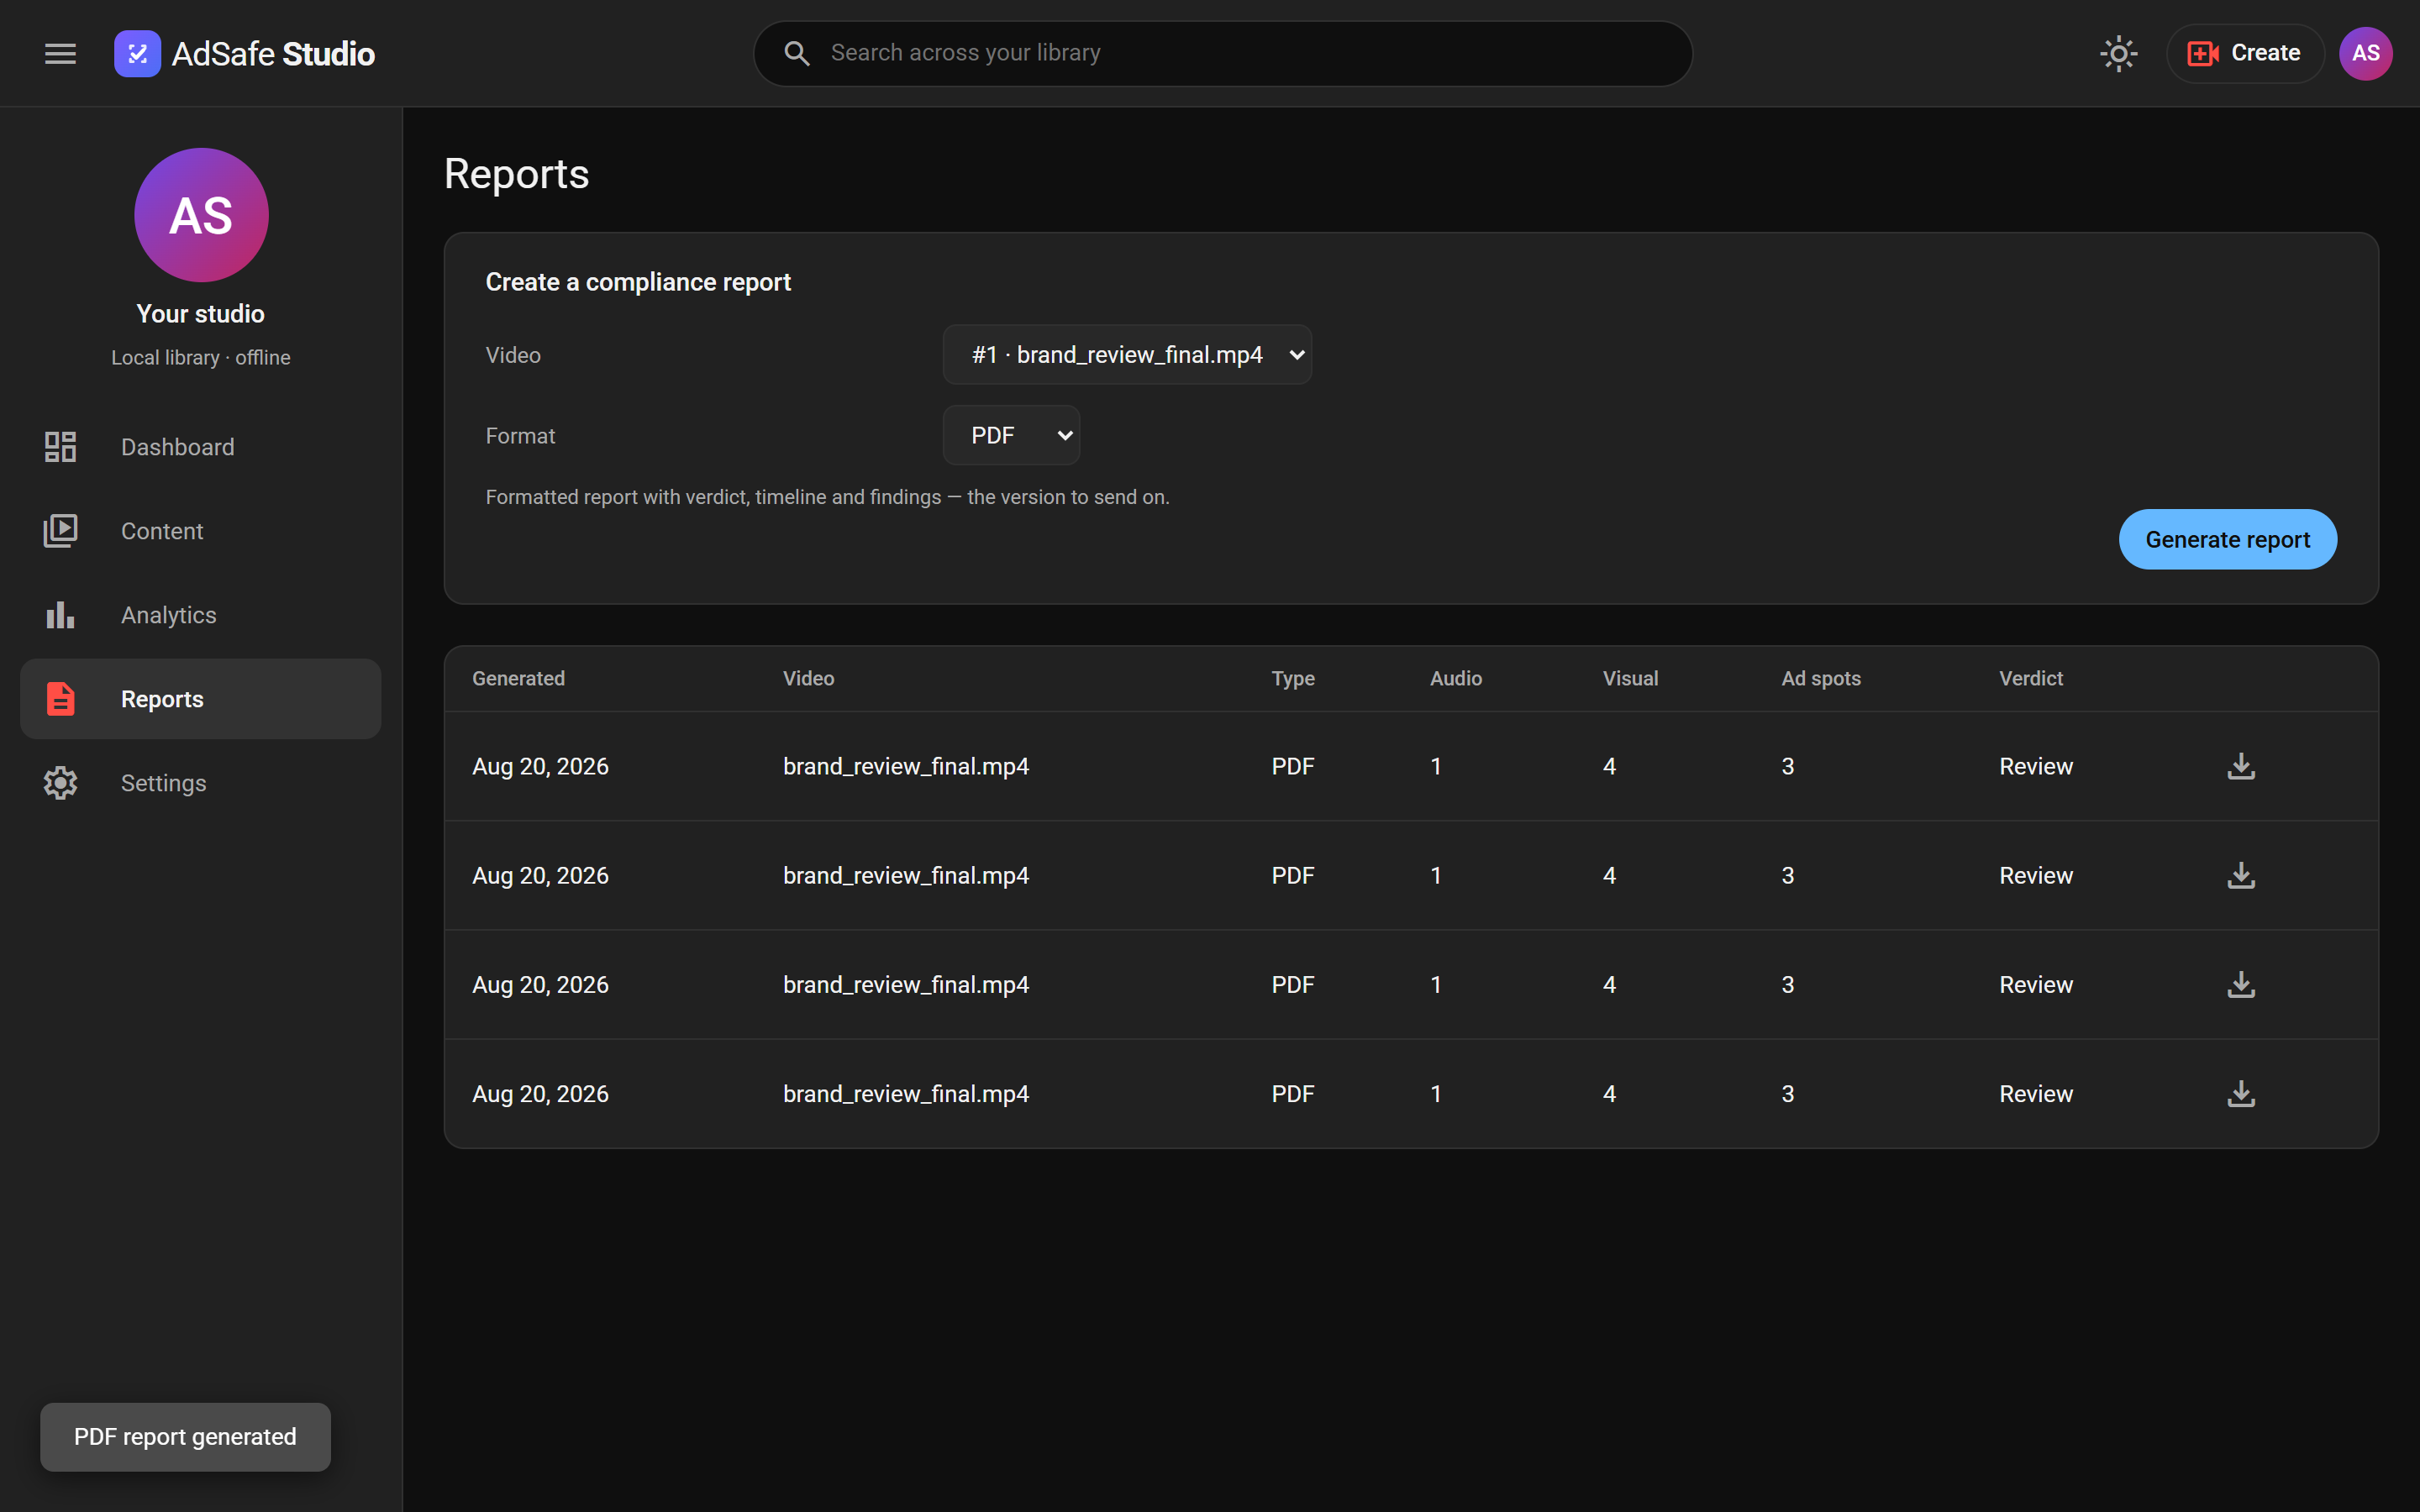
\includegraphics[width=0.95\textwidth]{Images/05-reports.png}
\caption{Reports Screen}
\end{figure}

\subsection{Settings Screen}

Allows the restricted dictionary, sampling rate, confidence threshold, detection resolution cap, analysis mode and model weights to be configured. The screen also reports which risk categories the currently loaded models are capable of detecting.

\begin{figure}[H]
\centering
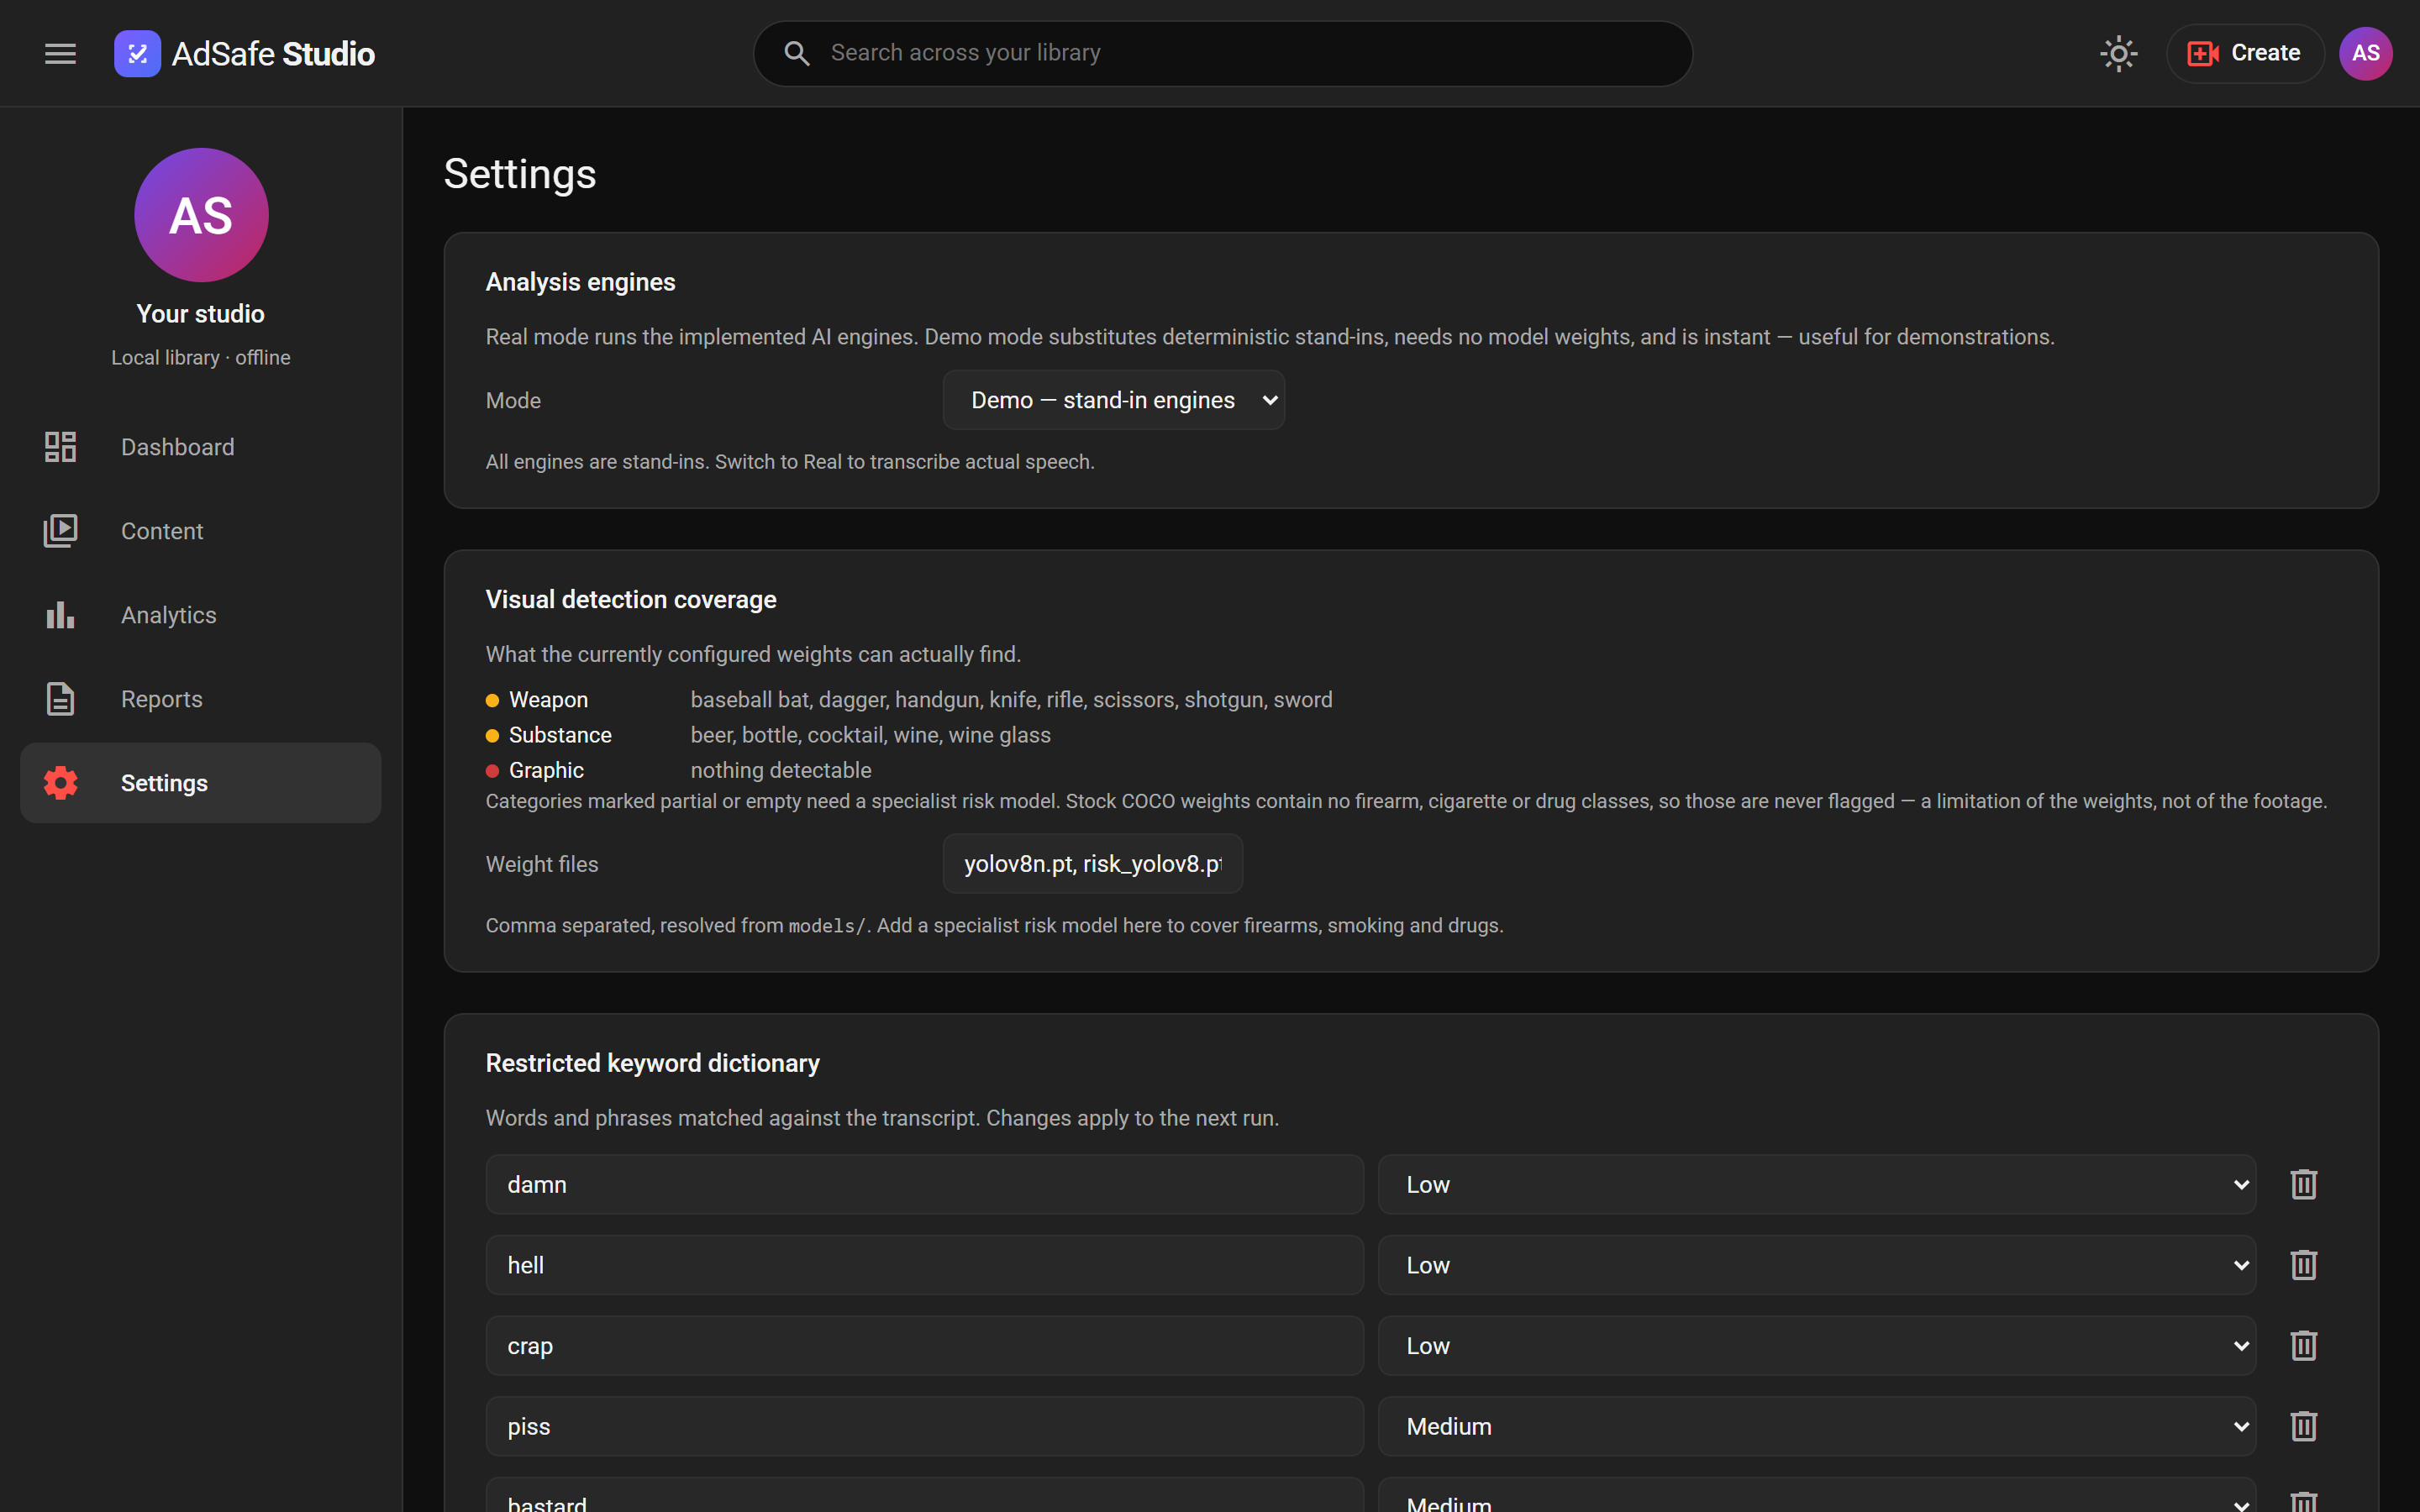
\includegraphics[width=0.95\textwidth]{Images/06-settings.png}
\caption{Settings Screen}
\end{figure}

\section{Design Advantages}

\begin{itemize}
\item Layered separation allows any engine to be replaced without altering the interface or the database.
\item Model class names are normalised at a single boundary, so changing models does not affect stored data.
\item Sequential execution avoids memory contention and database lock errors.
\item A single frame decode serving three consumers avoids redundant computation.
\item Database-level constraints reject invalid data regardless of the calling code.
\item Cascading deletion guarantees no orphaned findings.
\end{itemize}

\section{Chapter Summary}

This chapter described the four-layer architecture of the system and the responsibilities of its six modules. Two design decisions were recorded with their justification: sequential execution of the engines, and a single frame decode serving three consumers. The database design was presented in third normal form with its integrity constraints, and the seven interface screens were described.

%%%%%%%%%%%%%%%%%%%%%%%%%%%%%%%%%%%%%%%%%%%%%%%%%%
\chapter{Coding and Implementation}
%%%%%%%%%%%%%%%%%%%%%%%%%%%%%%%%%%%%%%%%%%%%%%%%%%

\section{Introduction}

This chapter describes the development environment, the organisation of the source, the implementation of each module, the coding standards adopted, and the validation and error handling mechanisms.

\section{Development Environment}

\subsection{Hardware Configuration}

\begin{table}[h]
\centering
\begin{tabular}{|p{5cm}|p{7cm}|}
\hline
\textbf{Component} & \textbf{Configuration} \\
\hline
Processor & Intel Core i5-1235U \\
\hline
Memory & 16 GB RAM \\
\hline
Storage & Solid state drive \\
\hline
Graphics & Integrated; no CUDA device \\
\hline
Operating System & Windows 11 \\
\hline
\end{tabular}
\caption{Hardware Configuration}
\end{table}

\subsection{Software Configuration}

\begin{table}[h]
\centering
\begin{tabular}{|p{5cm}|p{7cm}|}
\hline
\textbf{Component} & \textbf{Version} \\
\hline
Python & 3.12 \\
\hline
FastAPI with Uvicorn & Web framework and server \\
\hline
SQLite & 3.45 \\
\hline
faster-whisper & Speech recognition \\
\hline
Ultralytics YOLOv8 & Object detection \\
\hline
OpenCV & Image processing \\
\hline
ReportLab & PDF generation \\
\hline
React with Vite & Interface framework and build tool \\
\hline
Node.js & 22 \\
\hline
\end{tabular}
\caption{Software Configuration}
\end{table}

\section{Project Folder Structure}

The project is organised using the following directory structure.

\begin{verbatim}

specproj/
    backend/          FastAPI application and routes
    frontend/         React interface, components and pages
    src/
        config.py     Central paths and constants
        db/           Schema, connection handling, repository
        audio/        Extraction, transcription, keyword matching
        vision/       Sampling, detection, ad spots, overlay, tracking
        pipeline/     Orchestrator
        reports/      CSV, JSON and PDF exporters
        benchmark/    Accuracy evaluation harness
    benchmark/        Clip intake, labelling tool, evaluation CLI
    training/         Dataset preparation and model training
    tests/            Automated test suite
    data/             Videos, thumbnails, database, reports
    models/           Model weights

\end{verbatim}

\section{Module Description}

\subsection{Audio Module}

Extracts the audio track using a bundled encoder, so no system-wide media tool is required. Transcription produces word-level timestamps, which the findings table requires. The transcript is matched against the configured dictionary using word-boundary matching for single words and phrase matching for multi-word terms.

\subsection{Vision Module}

Loads one or more detection models and applies them to each sampled frame at two resolutions. Detections are merged, and duplicates arising from the two passes are removed by comparing class and overlap. Class names are normalised into risk categories at this boundary.

\subsection{Advertisement Placement Module}

Constructs a binary mask of unavailable regions from the detected objects and from local image texture, then locates the largest rectangles that fit inside the remaining area. Candidate surfaces are tracked across frames and retained only if they persist.

\subsection{Overlay Context Module}

Accumulates a running sum and sum of squares for each pixel, from which the temporal mean and variance are derived without retaining any frame. Regions that hold structure in the mean while remaining steadier than the surrounding scene are reported as overlay.

\subsection{Orchestration Module}

Selects the engine for each stage, executes the stages in order, reports progress, and records the engine that produced each finding.

\section{Coding Standards}

\begin{itemize}
\item Module and function names describe purpose rather than implementation.
\item Every module carries a docstring stating its responsibility.
\item Comments explain the reason for a decision rather than restating the code.
\item Constants are defined centrally rather than repeated.
\item Functions perform a single task.
\item Database access is confined to the repository layer.
\item Every defect is reproduced as a test before being corrected.
\end{itemize}

\section{Important Code Segments}

\subsection{Keyword Matching}

\begin{verbatim}

def match_transcript(words, dictionary, detection_model):
    flags = []
    for rule in dictionary:
        term = rule["word"].lower()
        for match in find_occurrences(words, term):
            flags.append({
                "timestamp_start": match.start,
                "timestamp_end": match.end,
                "word_flagged": term,
                "transcript_context": context_around(words, match),
                "severity": rule["severity"],
                "detection_model": detection_model,
            })
    return flags

\end{verbatim}

\subsection{Multi-Scale Detection}

\begin{verbatim}

def detect_frame(self, frame, timestamp):
    out = []
    for model in self._load():
        for imgsz in inference_scales(frame.shape[1],
                                      self.max_imgsz):
            out += self._predict_at(model, frame,
                                    imgsz, timestamp)
    return merge_scale_detections(out)

\end{verbatim}

\subsection{Largest Free Rectangle}

\begin{verbatim}

def largest_free_rectangle(free):
    best = (0, 0, 0, 0, 0)
    heights = [0] * free.shape[1]
    for y in range(free.shape[0]):
        for x in range(free.shape[1]):
            heights[x] = heights[x] + 1 if free[y][x] else 0
        area, x1, x2 = largest_in_histogram(heights)
        if area > best[0]:
            best = (area, x1, y - height + 1, x2, y)
    return best

\end{verbatim}

\subsection{Compliance Verdict}

\begin{verbatim}

def assess_compliance(video_id):
    audio_high = high_severity_terms(video_id)
    weapons = weapon_findings(video_id)
    overlay = overlay_context(video_id)

    if audio_high:
        return result("Restricted", spoken_reason(audio_high))
    if not weapons:
        return result("Monetizable", "No blocking findings.")
    if looks_like_rendered_gameplay(overlay):
        return result("Review", overlay_reason(weapons, overlay))
    return result("Restricted", weapon_reason(weapons))

\end{verbatim}

\section{Validation Checks}

Validation is applied at the interface, at the API boundary and in the database.

\begin{table}[h]
\centering
\begin{tabular}{|p{5cm}|p{6cm}|}
\hline
\textbf{Validation} & \textbf{Purpose} \\
\hline
File Format Validation & Accept only supported video formats \\
\hline
File Size Validation & Reject empty and oversized files \\
\hline
Duplicate Term Validation & Prevent repeated dictionary entries \\
\hline
Numeric Range Validation & Keep settings within workable limits \\
\hline
Analysis Mode Validation & Accept only known operating modes \\
\hline
Resolution Clamping & Constrain detection resolution to a usable range \\
\hline
Status Constraint & Restrict processing state to defined values \\
\hline
Severity Constraint & Restrict severity to Low, Medium or High \\
\hline
Category Constraint & Restrict risk category to defined values \\
\hline
\end{tabular}
\caption{Validation Checks}
\end{table}

\section{Error Handling}

\subsection{Media Errors}

A file that cannot be opened is rejected on ingestion with an explanatory message, and the uploaded copy is removed. A video containing no audio track is not treated as a failure: transcription is skipped, the reason is recorded, and visual analysis proceeds.

\subsection{Model Errors}

A model that cannot be loaded produces a message identifying the weight file and stating that a first-time download requires a network connection. Analysis is marked failed for that video only.

\subsection{Database Errors}

Foreign key enforcement and check constraints are applied at the database level, so invalid data is rejected regardless of the calling code. Write-ahead logging allows interface queries to proceed while analysis is writing.

\subsection{Application Errors}

Any unanticipated failure during analysis marks the video as failed rather than leaving it in a processing state indefinitely, and the interface reports the failure to the user.

\section{Sample Output Screens}

\subsection{Analysis Findings}

The video detail screen presents the compliance verdict with its reasoning, the finding counts, the audit timeline and the tables of individual findings.

\begin{figure}[H]
\centering
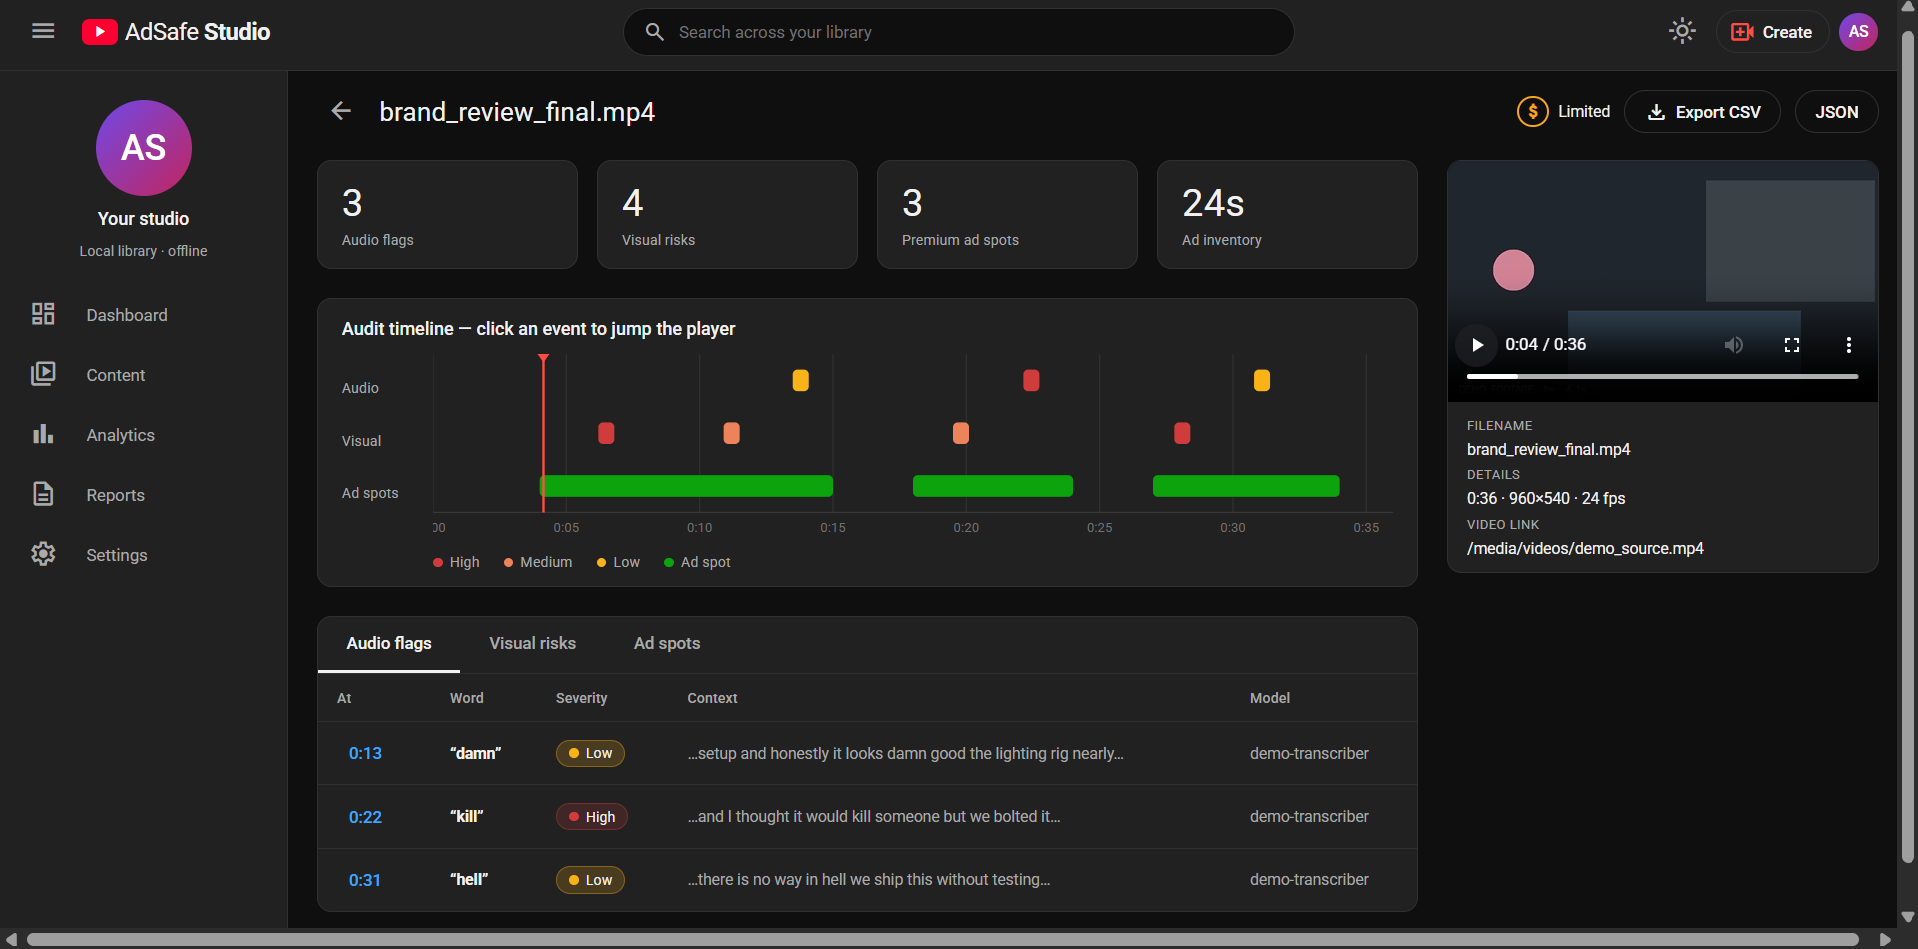
\includegraphics[width=0.95\textwidth]{Images/03-video-detail.png}
\caption{Analysis Findings Output}
\end{figure}

\subsection{Library Overview}

The content screen presents every analysed video with its monetization status.

\begin{figure}[H]
\centering
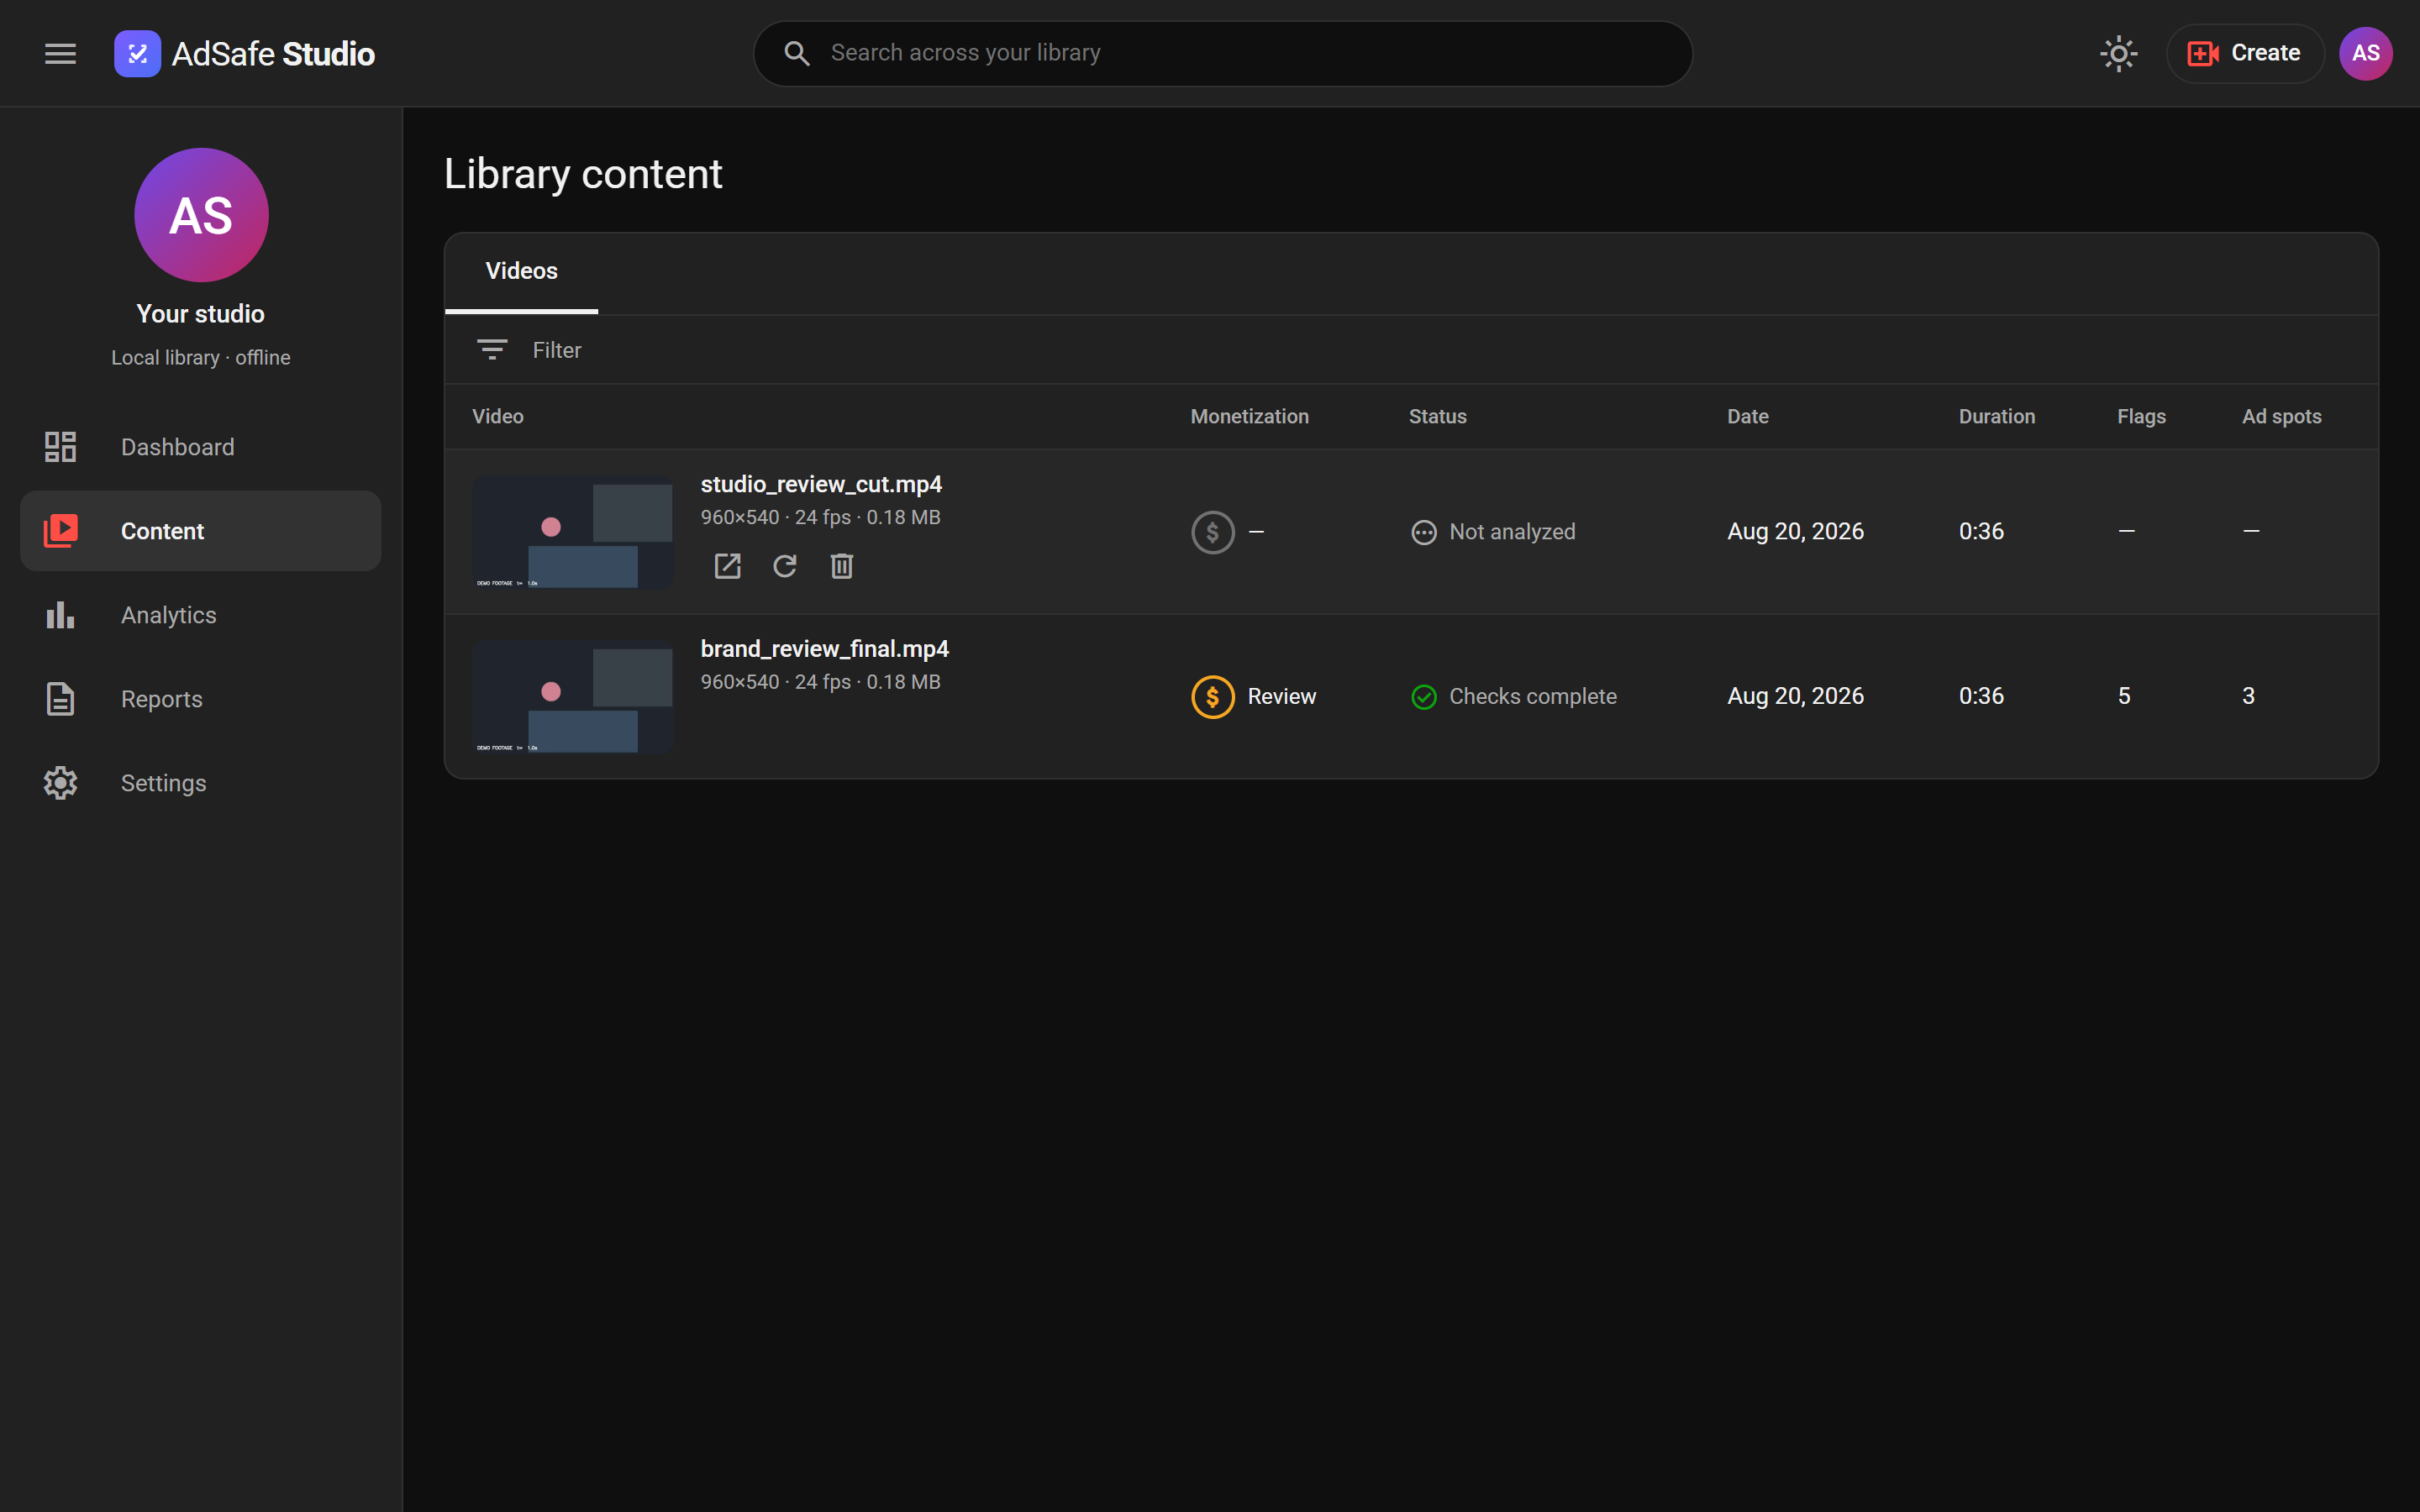
\includegraphics[width=0.95\textwidth]{Images/02-content.png}
\caption{Library Overview Output}
\end{figure}

\section{Implementation Advantages}

\begin{itemize}
\item The system operates entirely offline after the initial model download.
\item Every finding records the engine that produced it, so demonstration output cannot be mistaken for measured output.
\item Every verdict is accompanied by its reasoning.
\item Findings are named at the confidence the evidence supports.
\item The automated test suite contains 169 tests covering the data layer, the engines, the verdict logic and the API.
\item Each defect discovered during development is retained as a regression test.
\end{itemize}

\section{Chapter Summary}

This chapter described the implementation of the system: its development environment, source organisation, module implementations, coding standards and error handling. The validation strategy applies checks at three levels, so invalid data is rejected regardless of the path by which it arrives. The current implementation is supported by an automated suite of 169 tests, each defect found during development having been retained as a regression test.

\newpage
\centering
    \chapter*{Bibliography}

\begin{thebibliography}{9}

\bibitem{ref1}
Radford, A., Kim, J. W., Xu, T., Brockman, G., McLeavey, C., and Sutskever, I.,
\textit{Robust Speech Recognition via Large-Scale Weak Supervision}, OpenAI, 2022.

\bibitem{ref2}
Jocher, G., Chaurasia, A., and Qiu, J.,
\textit{Ultralytics YOLOv8}, 2023. Available: https://github.com/ultralytics/ultralytics

\bibitem{ref3}
Kuznetsova, A., Rom, H., Alldrin, N., Uijlings, J., Krasin, I., Pont-Tuset, J.,
Kamali, S., Popov, S., Malloci, M., Kolesnikov, A., Duerig, T., and Ferrari, V.,
\textit{The Open Images Dataset V4: Unified Image Classification, Object Detection,
and Visual Relationship Detection at Scale}, International Journal of Computer
Vision, 2020.

\bibitem{ref4}
Bradski, G.,
\textit{The OpenCV Library}, Dr. Dobb's Journal of Software Tools, 2000.

\bibitem{ref5}
Pressman, R. S. and Maxim, B. R.,
\textit{Software Engineering: A Practitioner's Approach}, 9th Edition,
McGraw-Hill Education, 2020.

\bibitem{ref6}
Sommerville, I.,
\textit{Software Engineering}, 10th Edition, Pearson Education, 2016.

\bibitem{ref7}
Elmasri, R. and Navathe, S. B.,
\textit{Fundamentals of Database Systems}, 7th Edition, Pearson, 2016.

\bibitem{ref8}
YouTube Help,
\textit{Advertiser-friendly content guidelines}, Google LLC.
Available: https://support.google.com/youtube/answer/6162278

\end{thebibliography}

\end{document}
